\documentclass[a4paper,UKenglish,cleveref, autoref, thm-restate]{lipics-v2021}

\usepackage{amsmath}
\usepackage{amssymb}
\usepackage{algorithm}
\usepackage[noend]{algpseudocode}
%\usepackage [pagewise]{lineno}
%\linenumbers
\usepackage{tikz}
\usepackage{bm}
\usepackage{graphicx}
\usepackage{amsfonts}
\usepackage[utf8]{inputenc}
\usepackage{stmaryrd}
\usepackage{url}
%\usepackage{sidecap}

\EventEditors{Florin Manea and Alex Simpson}
\EventNoEds{2}
\EventLongTitle{30th EACSL Annual Conference on Computer Science Logic (CSL 2022)}
\EventShortTitle{CSL 2022}
\EventAcronym{CSL}
\EventYear{2022}
\EventDate{February 14--19, 2022}
\EventLocation{G\"{o}ttingen, Germany (Virtual Conference)}
\EventLogo{}
\SeriesVolume{216}
\ArticleNo{7}

\usetikzlibrary{positioning,chains,fit,shapes,calc}
%\linenumbers
\setlength{\intextsep}{0.7\baselineskip}
\newcommand{\vars}{\mathit{vars}}
\newcommand{\allterms}{\mathit{ter}}
\newcommand{\terms}{\tau}
\newcommand{\dom}{\mathit{dom}}
\newcommand{\pred}{\mathit{def}}
\newcommand{\defs}{\mathit{freshdefs}}
\newcommand{\lfp}{\mathit{lfp}}
\newcommand{\wim}[1]{\textbf{Wim: #1}}
\newcommand{\gonz}[1]{\textbf{Gonz: #1}}
\newcommand{\gen}{\ensuremath{\mathit{gen}}}
\newcommand{\confs}{\mathit{confs}}
\newcommand{\compatible}{\mathit{comp}}
\newcommand{\enforce}{\triangleleft}
\newcommand{\mean}{\mathit{mean}}
\newcommand{\img}{\mathit{img}}
\newcommand{\mcg}{\mathit{mcg}}
\newcommand{\au}{\texttt{au}}
\newcommand{\MWM}{\texttt{MWM}}
\newcommand{\dau}{\texttt{dau}}
\newcommand{\score}{\texttt{score}}
\newcommand{\lcg}{\textsc{lcg} }
\newcommand{\msg}{\textsc{msg} }
\newcommand{\spc}{\hspace*{3ex}}

\nolinenumbers

\title{Anti-unification of Unordered Goals}

\author{Gonzague Yernaux}{University of Namur - Faculty of Computer Science (Belgium)\\Namur Digital Institute}{gonzague.yernaux@unamur.be}{https://orcid.org/0000-0001-6430-8168}{}
\author{Wim Vanhoof}{University of Namur - Faculty of Computer Science (Belgium)\\Namur Digital Institute}{wim.vanhoof@unamur.be}{https://orcid.org/0000-0003-3769-6294}{}

\authorrunning{G. Yernaux and W.\, Vanhoof} 

\Copyright{Gonzague Yernaux and Wim Vanhoof}

\ccsdesc[500]{Theory of computation~Constraint and logic programming}

\keywords{Anti-unification, Logic programming, NP-completeness, Time complexity, Algorithms, Inductive logic programming}
\category{} %optional, e.g. invited paper

%\relatedversion{https://arxiv.org/abs/2107.00341} %optional, e.g. full version hosted on arXiv, HAL, or other respository/website
%\relatedversion{A full version of the paper is available at \url{...}.}

%\supplement{}%optional, e.g. related research data, source code, ... hosted on a repository like zenodo, figshare, GitHub, ...

\begin{document}   

	\maketitle 
	\begin{abstract}
		Anti-unification in logic programming refers to the process of capturing common syntactic structure among given goals, computing a single new goal that is more general called a generalization of the given goals. Finding an arbitrary common generalization for two goals is trivial, but looking for those common generalizations that are either as large as possible (called largest common generalizations) or as specific as possible (called most specific generalizations) is a non-trivial optimization problem, in particular when goals are considered to be \textit{unordered} sets of atoms. In this work we provide an in-depth study of the problem by defining two different generalization relations. We formulate a characterization of what constitutes a most specific generalization in both settings. While these generalizations can be computed in polynomial time, we show that when the number of variables in the generalization needs to be minimized, the problem becomes NP-hard. We subsequently revisit an abstraction of the largest common generalization when anti-unification is based on injective variable renamings, and prove that it can be computed in polynomially bounded time. 
	\end{abstract}


	%%%%%%%%%%%%%%%%%%%%%%%%%%%%%%%%%%%%%%%%%%%%%%%%%%%
	%%%%%%%%%%%%%%%%%%%%%%%%%%%%%%%%%%%%%%%% ABSTRACT
	%%%%%%%%%%%%%%%%%%%%%%%%%%%%%%%%%%%%%%%%%%%%%%%%%%%
	

	
	%%%%%%%%%%%%%%%%%%%%%%%%%%%%%%%%%%%%%%%%%%%%%%%%%%%
	%%%%%%%%%%%%%%%%%%%%%%%%%%%%%%%%%%%%%%%% Intro
	%%%%%%%%%%%%%%%%%%%%%%%%%%%%%%%%%%%%%%%%%%%%%%%%%%%
	% !TEX root = 0-qqQQmain.tex

\section{Introduction}


The success of the collider particle physics program, whose main
player today is the Large Hadron Collider (LHC) at CERN, relies
heavily on our ability to model with high precision and accuracy the
scattering of high energetic protons in Quantum Chromodynamics (QCD).
Thanks to asymptotic freedom and the factorization properties of QCD,
this intrinsically non-perturbative problem can be treated with
perturbative methods, supplemented by non-perturbative information about
the distribution of partons in the proton. Within this picture, an important
role is played by higher order perturbative QCD calculations, which allow
for a reliable and precise description of a wide range of collider processes
and observables.

Thanks to a concerted effort in the high-energy community over the
last few years, it is currently possible to compute predictions for
many interesting reactions to second order in the strong coupling
expansion, $i.e.$ to what is usually referred to as
next-to-next-to-leading order (NNLO). 
This has required, on the one hand, 
major advances in computational techniques
for multi-loop scattering amplitudes~\cite{Tkachov:1981wb,Chetyrkin:1981qh,Hodges:2009hk,Gluza:2010ws,Ita:2015tya,Larsen:2015ped,Bohm:2017qme,Badger:2016uuq,vonManteuffel:2014ixa,Peraro:2016wsq,Peraro:2019svx,Guan:2019bcx,Pak:2011xt,Abreu:2019odu,Heller:2021qkz,Kotikov:1990kg,Bern:1993kr,Remiddi:1997ny,Gehrmann:1999as,Papadopoulos:2014lla,Dixon:1996wi,Henn:2013pwa,Primo:2016ebd,Goncharov,Remiddi:1999ew,Goncharov:2001iea,Goncharov:2010jf,Brown:2008um,Ablinger:2013cf,Panzer:2014caa,Duhr:2011zq,Duhr:2012fh,Duhr:2019tlz},
which, notably, have recently made it possible to compute
various $2 \to 3$ processes up to two loops in QCD~\cite{Badger:2017jhb,Abreu:2017hqn,Abreu:2018aqd,Abreu:2018zmy,Abreu:2018jgq,Abreu:2019rpt,Abreu:2020cwb,Chicherin:2018yne,Chicherin:2019xeg,Chawdhry:2020for,DeLaurentis:2020qle,Chawdhry:2018awn,Abreu:2020xvt,Agarwal:2021grm,Badger:2021nhg,Abreu:2021fuk,Agarwal:2021vdh,Chawdhry:2021mkw,Badger:2021imn,Gehrmann:2015bfy,Papadopoulos:2015jft,Gehrmann:2018yef,Chicherin:2018mue,Chicherin:2020oor}.
On the other hand, the use of these amplitudes to perform phenomenological
studies for the relevant processes at NNLO~\cite{Chawdhry:2019bji,Kallweit:2020gcp,Chawdhry:2021hkp,Czakon:2021mjy} has required the
development of so-called subtraction or slicing frameworks~\cite{GehrmannDeRidder:2005cm,Czakon:2010td,Caola:2017dug,Magnea:2018hab,Herzog:2018ily,DelDuca:2016ily,Cacciari:2015jma,Catani:2007vq,Gaunt:2015pea,Boughezal:2015dva}
to properly deal with the intricate IR divergences that appear in QCD reactions. 

Beyond NNLO, predictions at third order in the
perturbative couplings, i.e.\ at N$^3$LO, are
known only for a handful of important LHC processes~\cite{Anastasiou:2015vya,Duhr:2019kwi,
Dulat:2018bfe,Mistlberger:2018etf,Dreyer:2016oyx,Dreyer:2018qbw,
Billis:2021ecs,Chen:2021isd,Chen:2021vtu}. 
In particular, N$^3$LO results are currently available only for reactions that
require at most three-point three-loop integrals.
Given the remarkable success of the
experimental program at the LHC, it is desirable to extend these
calculations to more complex processes. A particularly interesting
one is di-jet production.  In fact, jets are ubiquitous at
hadron colliders, so understanding their dynamics is of great
interest.
Moreover, di-jet production is the first massless $2\to2$
process that has a non-trivial colour structure. This makes it an
ideal ground for studying the structure of perturbative QCD. For
example, it is by now well known that when four or more coloured
partons interact, starting at the three-loop order, non-trivial
colour correlations can affect the pattern of IR divergences,
generating new structures~\cite{Almelid:2015jia} beyond the standard dipole
formula~\cite{Sterman:2002qn,Aybat:2006wq,Aybat:2006mz,Becher:2009cu,Gardi:2009qi,Becher:2009qa,Dixon:2009gx}. Also, the
non-trivial colour structure may create subtle violations of the
factorization framework that is at the very core of theoretical
predictions at hadronic
colliders~\cite{Catani:2011st,Forshaw:2012bi,Forshaw:2006fk,Becher:2021zkk}.
This makes jet production at hadronic colliders an extremely interesting
process to investigate at higher orders. 

A key ingredient for the study of jet production at N$^3$LO is
provided by the virtual three-loop corrections to the scattering
amplitudes for the production of two jets in massless QCD.  Modulo
crossings, there are three main partonic channels that need to be
computed: four-gluon scattering, the scattering of two quarks and two
gluons, and the scattering of four quarks.  All ingredients necessary
for the calculation of the two-loop QCD corrections to these processes have
been known for a long time~\cite{Smirnov:1999gc,Tausk:1999vh,Glover:2001af,Anastasiou:2002zn,Glover:2003cm}, which 
have made it possible to compute the relevant scattering amplitudes~\cite{Anastasiou:2000kg,Bern:2003ck,Glover:2004si,DeFreitas:2004kmi}. Also, in view of extending these
calculations to three loops, results for the two loop helicity
amplitudes up to order $\epsilon^2$ have been
obtained~\cite{Ahmed:2019qtg}.  For what concerns the three loop
results, instead, the relevant master integrals have been computed in
ref.~\cite{Henn:2020lye}, and have then been used to obtain the first
three loop results for $2 \to 2$ scattering amplitudes in
supersymmetric theories~\cite{Henn:2016jdu,Henn:2019rgj}.  More
recently also the first three loop corrections to the production of
two photons in full QCD have been obtained~\cite{Caola:2020dfu}.

In this paper, we move one step further and consider one of the three classes of partonic processes  listed above, 
namely the scattering of four massless quarks. This particular process is interesting not only
because it allows us, for the first time, to check the full structure of IR divergences at three loops in QCD, 
but also because it involves two external spinor structures. In fact, this property makes the use of the standard form factors
method for the calculation of the helicity amplitudes particularly cumbersome, due to the fact that the  $\gamma$-algebra does not
close in  $d$ space-time dimensions. For the calculation of the helicity amplitudes we then make use of
a different approach, recently described in refs~\cite{Peraro:2019cjj,Peraro:2020sfm}, which allows us to calculate the helicity amplitudes
in a simpler way, corresponding to the 't Hooft-Veltman scheme (tHV)~\cite{tHooft:1972tcz} for the processes considered here.\footnote{See also ref.~\cite{Heller:2020owb} for an application of similar ideas in the case of a chiral theory, and ref.~\cite{Chen:2019wyb} for an alternative approach.} 
In doing this, we also expose some
subtleties in the usual approach to compute helicity amplitudes in 
tHV with the standard form factor method.
The rest of the paper is organised as follows. 
We start in section~\ref{Kinematics} by establishing the notation for the calculation of the
fundamental partonic channel $q\bar{q} \to Q \bar{Q}$, from which all other channels can by obtained by crossing.
We continue in section~\ref{The Scattering Amplitude},
where we describe the colour and tensor decomposition  of the scattering amplitude, and show how to 
efficiently compute the helicity amplitudes without considering evanescent Lorentz structures.
In section~\ref{computation} we provide details on our computational set up,
and in section~\ref{subtraction} we discuss the renormalisation and the infrared structure of the three-loop scattering amplitudes.
In section~\ref{results} we discuss our final results for the main partonic channel.
In section~\ref{extra_results} we then explain how to obtain all other partonic channels from our calculation, both for quarks of equal and different flavour.
Finally we conclude in section~\ref{conclusions}.  In 
appendices~\ref{sec:appB} and~\ref{sec:appA}
we provide some details on the structure of infrared divergences up at three loops, in particular focusing on the explicit derivation of the quadrupole terms, which appear for the first time with the scattering of at least four coloured partons at three loops.
In appendix~\ref{sec:appC}, we review the analytical continuation of the amplitudes to different regions of phase space.

	
	%%%%%%%%%%%%%%%%%%%%%%%%%%%%%%%%%%%%%%%%%%%%%%%%%%%
	%%%%%%%%%%%%%%%%%%%%%%%%%%%%%%%%%%%%%%%% Préliminaires
	%%%%%%%%%%%%%%%%%%%%%%%%%%%%%%%%%%%%%%%%%%%%%%%%%%%
	\section{Preliminaries}
\label{sec:preliminaries}
% \paragraph{Locally Differentially Private (LDP).}
\subsection{Locally Differentially Private (LDP)}
% \label{subsec:ldp}
Suppose $\svbx \in \cX$ is some user's data that must remain private.  A privatization mechanism $q$ is a randomized mapping that maps $\svbx \in \cX$ to $\svbz \in \cZ$ with probability $q(\svbz|\svbx)$ where $\cZ$ can be arbitrary. The user transmits $\svbz \sim q(\cdot|\svbx)$, i.e., a privatized version of $\svbx$ to the server. Further, $q$ is $\varepsilon$-LDP if 
\begin{align}
    \forall \svbx, \svbx' \in \cX, \svbz \in \cZ, ~ q(\svbz|\svbx) \leq e^{\varepsilon} q(\svbz|\svbx')  \label{eq:ldp}
\end{align}
and $q$ is $(\varepsilon, \delta)$-LDP if $\forall \svbx, \svbx' \in \cX, Z \subseteq \cZ,$
$$\sum_{\svbz \in Z} q(\svbz|\svbx) \leq e^{\varepsilon} \sum_{\svbz \in Z} q(\svbz|\svbx') + \delta.$$
% \begin{align}
%      \sum_{\svbz \in Z} q(\svbz|\svbx) \leq \exp(\varepsilon) \sum_{\svbz \in Z} q(\svbz|\svbx') + \delta. \label{eq:ldp2}
% \end{align}
Here, we focus on $\varepsilon$-LDP mechanisms where $\varepsilon \geq 1$.

% From now onwards, we will denote an $\varepsilon$-LDP $q$ by $q^\varepsilon$.

% \paragraph{Shared Randomness.}
\subsection{Shared Randomness}
\label{subsec:shared_randomness}
% \begin{remark}
Here, we allow $\varepsilon$-LDP mechanisms to use \emph{shared randomness}. That is, $q$ can depend on a random variable $\svbu \in \cU$ that is known to both the user and the server (but $\svbu$ is independent of $\svbx$). The corresponding $\varepsilon$-LDP constraint is
$$\forall \svbx, \svbx' \in \cX, \svbz \in \cZ, \svbu \in \cU, ~ q(\svbz|\svbx, \svbu) \leq \exp(\varepsilon)q(\svbz|\svbx', \svbu). $$
The server wishes to reconstruct $\svbx$ from $\svbz$ and the corresponding estimator is allowed to implicitly depend on $\svbu$.
% We allow the estimator of $\svbx$ at the server to implicitly depend on $\svbu$. 
However, for simplicity, we suppress the dependence on $\svbu$ in our notation. In practice, shared randomness can be achieved via downlink communication, that is, the server generates $\svbu$ (e.g., a random seed) and communicates it to the user. Further, we note that such shared randomness can be established well before the advent of any private data\footnote{Quantifying the amount of such shared randomness required remains an open question. See Section \ref{sec:conclusion}.}.
% \end{remark}

%\subsection{Shared Randomness}
\subsection{\texorpdfstring{PrivUnit$_2$}{PrivUnit}}
% \label{subsec:privunit}
% \paragraph{PrivUnit$_2$.}
The $\PrivUnit$ mechanism $\qPU$, proposed by \cite{BDFKR2018}, is an $\varepsilon$-LDP sampling scheme when the input alphabet $\cX$ is the $d-$dimensional unit $\ell_2$ sphere $\sphere^{d-1}$. Formally, given a vector $\svbx \in \sphere^{d-1}$, $\PrivUnit$ draws a random vector $\svbz$ 
% from $\sphere^{d}$ with the following conditional probability:
from a spherical cap $\{\svbz \in \sphere^{d-1} \mid
\lan \svbz, \svbx  \ran \ge \gamma\}$ with probability $p_0$ or from its complement $\{\svbz \in \sphere^{d-1} \mid \lan \svbz, \svbx \ran < \gamma\}$  with probability $1 - p_0$, 
% \begin{align}\label{eq:q_ss}
%     q^{\varepsilon}(\svbz|\svbx) \coloneqq \begin{cases}
%     \frac{e^{\varepsilon}}{{\binom{d-1}{s-1}}e^{\varepsilon}+{\binom{d-1}{s}}} & \text{if}\ \svbz : \lan \svbz, \svbx  \ran \ge \gamma
%     \\[10pt]
%     \frac{1}{{\binom{d-1}{s-1}}e^{\varepsilon}+{\binom{d-1}{s}}} & \text{if}\ \svbz : \lan \svbz, \svbx  \ran < \gamma
%     \end{cases}
% \end{align}
where $\gamma \in [0, 1]$ and $p_0  \geq 1/2$ are parameters (depending on $\varepsilon$ and $d$) that trade accuracy and privacy (see Appendix \ref{appendix:privunit}). In other words, $\qPU$ is as follows:
\begin{align}
    \qPU(\svbz | \svbx)   =   
    \begin{cases}
        \dfrac{2 p_0}{A(1,d)I_{1-\gamma^2}(\frac{d-1}{2},\frac{1}{2})} \hspace{10pt} \text{if}\ \langle \rvbx, \rvbz \rangle \geq \gamma \\[10pt]
       \dfrac{2(1-p_0)}{2A(1,d)  -  A(1,d)I_{1-\gamma^2}(\frac{d-1}{2},\frac{1}{2})} \hspace{6pt} \text{otherwise}
    \end{cases}
\end{align}
where $A(1,d)$ denotes the area of $\sphere^{d-1}$ and $I_x(a,b)$ denotes the regularized incomplete beta function. The estimator of the $\PrivUnit$ mechanism (denoted by $\hat{\svbx}^{\texttt{pu}}$) is obtained by dividing every coordinate of $\svbz$ by $m_{\texttt{pu}}$ i.e., $\hat{\svbx}^{\texttt{pu}} \coloneqq \svbz/m_{\texttt{pu}}$ where 
\begin{align}
    m_{\texttt{pu}} \coloneqq  \frac{(1 - \gamma^2)^\alpha}{2^{d-2} (d - 1)}
  \left[\frac{p_0}{B(1; \alpha,\alpha) - B(\tau; \alpha,\alpha)}
     - \frac{1 - p_0}{B(\tau; \alpha, \alpha)}\right]
  \label{eq:m}
\end{align}
%\begin{align}
    %m_{\texttt{pu}}   \coloneqq    \frac{(1   -   \gamma^2)^\alpha}{2^{d-2} (d   -   1)}
  %  \left[\frac{p_0}{B(1; \alpha,\alpha)   -   B(\tau; \alpha,\alpha)}
     %  -   \frac{1 - p_0}{B(\tau; \alpha, \alpha)}\right]
  %\label{eq:m}
%\end{align}
with $\alpha = (d-1)/2$, $\tau = (1+\gamma)/2$, and $B(x;\alpha,\beta)$ denoting the incomplete beta function. The estimator $\hat{\svbx}^{\texttt{pu}}$ is (a) unbiased i.e., $\Expectation[\hat{\svbx}^{\texttt{pu}} | \svbx] = \svbx$, (b) has order-optimal utility i.e., $\E[\ltwo{\hat{\svbx}^{\texttt{pu}} - \svbx}^2] = \Theta\lp
   \frac{d}{\min\lp\varepsilon, (e^\varepsilon-1)^2, d\rp}\rp$, and (c) achieves the best known constants for mean estimation. See Appendix \ref{appendix:privunit} for more details on $\PrivUnit$.

% In order to have an unbiased estimator, the vector $\svbz$ is scaled by $1/m$ where 
% \begin{align}
%     m \coloneqq \frac{(1 - \gamma^2)^\alpha}{2^{d-2} (d - 1)}
%     \left[\frac{p}{B(1; \alpha,\alpha)   -   B(\tau; \alpha,\alpha)}
%        -   \frac{1 - p}{B(\tau; \alpha, \alpha)}\right]
%   \label{eq:m}
% \end{align}
% with $\alpha = (d-1)/2$, $\tau = (1+\gamma)/2$, and $B(x;\alpha,\beta)$ denoting the incomplete beta function.
% More precisely, the estimator of the $\PrivUnit$ mechanism (denoted by $\hat{\svbx}^{\texttt{pu}}$) is defined as $\svbx/m$ and is such that $\Expectation[\hat{\svbx}^{\texttt{pu}} | \svbx] = \svbx$.
% For appropriate choices of the spherical cap level $\gamma$ and more details about the $\PrivUnit$ mechanism, see Appendix. 


\subsection{Subset Selection}
% \label{subsec:subsetselection}
% \paragraph{Subset Selection.}
The $\SubsetSelection$ mechanism $\qSS$, proposed by \cite{YB18}, is an $\varepsilon$-LDP sampling scheme when the input alphabet $\cX$ can take $d$ different values.
% $\cX$ is $[d] = \{1,\cdots,d\}$. 
Without loss of generality, let 
$\cX \coloneqq \lbp e_1, e_2,...,e_d \rbp$, where $e_j \in \{0, 1\}^d$ is the $j^{th}$ standard unit vector, i.e., the one-hot encoding of $j$.
The output alphabet $\cZ$ is the set of all $d$-bit binary strings with Hamming weight $s \coloneqq \lceil \frac{d}{1+e^{\varepsilon}}\rceil$, i.e.,
\begin{align*}
\textstyle
\cZ = \lbp \svbz = (z^{(1)}, \cdots ,z^{(d)}) \in \{0, 1\}^d: \sum_{i=1}^d z^{(i)} = s \rbp.
\end{align*}
Given $\svbx \in \cX$,  $\SubsetSelection$ maps it to $\svbz \in \cZ$ with the following conditional probability:
% Given a symbol $x \in [d]$, $\SubsetSelection$ first maps $x$ to its one-hot encoding
% $\svbx = (x^{(1)}, \cdots ,x^{(d)}) \in \{0, 1\}^d$ and then maps $\svbx$ to $\svbz \in \cZ$ with the following conditional probability:
\begin{align}\label{eq:q_ss}
    \qSS(\svbz|\svbx) \coloneqq \begin{cases}
    \frac{e^{\varepsilon}}{{ \binom{d-1}{s-1} }e^{\varepsilon}+{ \binom{d-1}{s} }} & \text{if}\ \svbz \in \cZ_{\svbx}
    \\[10pt]
    \frac{1}{{ \binom{d-1}{s-1} }e^{\varepsilon}+{ \binom{d-1}{s} }} & \text{if}\ \svbz \in \cZ \setminus \cZ_{\svbx}
    \end{cases}
\end{align}
where $\cZ_{\svbx} = \lbp \svbz = (z^{(1)}, \cdots ,z^{(d)}) \in \cZ : z^{(x)} = 1 \rbp$ is the set of elements in $\cZ$ with $1$ in the $x^{th}$ location. The estimator of the $\SubsetSelection$ mechanism (denoted by $\hat{\svbx}^{\texttt{ss}}$) is obtained by subtracting $b_{\texttt{ss}}$ from every component of $\svbz$ and dividing every component of the result by $m_{\texttt{ss}}$ i.e., $\hat{\svbx}^{\texttt{ss}} \coloneqq (\svbz - b_{\texttt{ss}})/m_{\texttt{ss}}$ where 
\begin{align}\label{eq:m_ss}
    m_{\texttt{ss}} \coloneqq \frac{s(d  -  s)(e^{\varepsilon}-1)}{(d  -  1)(s(e^{\varepsilon}  -  1)+d)},\  b_{\texttt{ss}} \coloneqq  \frac{s((s  -  1)e^{\varepsilon} +(d  -  s))}{(d  -  1)(s(e^{\varepsilon}  -  1)+d)}.
\end{align}
% \begin{align}\label{eq:m_ss}\textstyle
%     m_{\texttt{ss}}   \coloneqq   \frac{s(d   -   s)(e^{\varepsilon}-1)}{(d   -   1)(s(e^{\varepsilon}   -   1)+d)},
%     \quad b_{\texttt{ss}}   \coloneqq   \frac{s((s   -   1)e^{\varepsilon} +(d   -   s))}{(d   -   1)(s(e^{\varepsilon}   -   1)+d)}.
% \end{align}
% first maps it to its one-hot encoding $\svbx = (x^{(1)}, \cdots ,x^{(d)}) \in \{0, 1\}^d$. Then, with $t \coloneqq \lceil \frac{d}{1+e^{\varepsilon}}\rceil$, 
The estimator $\hat{\svbx}^{\texttt{ss}}$ is (a) unbiased i.e., $\Expectation[\hat{\svbx}^{\texttt{ss}} | \svbx] = \svbx$, (b) has optimal utility i.e., $\E[\ltwo{\hat{\svbx}^{\texttt{ss}} - \svbx}^2] = \Theta\lp \frac{d}{\min\lp e^{\varepsilon}, \lp e^{\varepsilon}-1 \rp^2, d \rp}\rp$ and (c) achieves the best known constants for frequency estimation. See Appendix \ref{appendix:ss} for more details on $\SubsetSelection$.
	
	%%%%%%%%%%%%%%%%%%%%%%%%%%%%%%%%%%%%%%%%%%%%%%%%%%%
	%%%%%%%%%%%%%%%%%%%%%%%%%%%%%%%%%%%%%%%% 
	%%%%%%%%%%%%%%%%%%%%%%%%%%%%%%%%%%%%%%%%%%%%%%%%%%%
	\section{Large and Specific Generalizations}\label{section-relation-1}

In this section we prove that msg's and lcg's as defined above can be computed with polynomial-time algorithms. First, we need the concept of a \textit{variabilization} which is basically a function mapping couples of terms to new variables. 

\begin{definition}%[Variabilization function]
	Given a context $\langle X, \mathcal{V}, \mathcal{F}, \mathcal{Q}\rangle$, let
	$V\subset \mathcal{V}$ denote a set of variables. A function $\Phi_V : \mathcal{T}^2\mapsto\mathcal{V}\cup X$ is called a \emph{variabilization function} if, for any $(t_1, t_2)\in\mathcal{T}^2$ it holds that if $\Phi_V(t_1,t_2) = v$, then
	$(1)\; v \notin V,\;(2)\;\nexists (t_1', t_2') \in \mathcal{T}^2 : (t_1', t_2') \neq (t_1, t_2) \wedge \Phi_V(t_1', t_2') = v, \; (3) \; v \in X \Leftrightarrow t_1 = t_2\in X$ and in that case, $v = t_1 = t_2$.
\end{definition}

Note that a variabilization function $\Phi_V$ introduces a new variable (not present in $V$) for any couple of terms, except when the terms are the same constant. It can thus be seen as a way to introduce new variable names when going through the process of anti-unifying two goals. In what follows, when manipulating goals $G_1$ and $G_2$, we will use $\Phi_{\vars(G_1\cup G_2)}$ to represent an arbitrary variabilization function. If the goals at hand are clearly identified from the context, we will abbreviate the notation to $\Phi$. In most upcoming examples we will use applications of $\Phi$ (e.g. $\Phi(X,Y), \Phi(t(X), 5),\dots$) rather than coined variable names (e.g. $V_1, V_2,\dots$) when an anti-unification operator is -- ostensibly or not -- at work.

Algorithm~\ref{algo-rel-1-lcg} shows the intuitive solution for computing a lcg with two goals $G_1$ and $G_2$ (where we suppose $|G_1|\le|G_2|$) as input. In the algorithm, $\au_\leqslant(A_1,A_2)$ denotes the use of a function that outputs a $\leqslant$-common generalization on the atomic level for atoms $A_1$ and $A_2$ with respect to relation $\leqslant$. In our development we will call such functions \textit{anti-unification operators}. %, defined as follows. 
As stated in the following observation, such operators exist for our relations.

\begin{algorithm}[hbtp]
	\caption{Computing a lcg $G$ for goals $G_1$ and $G_2$ with generalization relation $\leqslant$} 
	\label{algo-rel-1-lcg}
	\begin{algorithmic}
		\State $G = \{\}, R = \{\}$ 
		\For {each ($A_1 \in G_1$)}
		\For {each ($A_2 \in G_2\setminus R$)}
		\State $A_1'$ = $\au_\leqslant(A_1, A_2)$
		\If{$A_1' \neq \bot$}				
		\State $G \gets G\cup A_1'$
		\State $R \gets R\cup A_2$
		\State \textbf{break} out of the inner loop
		\EndIf
		\EndFor
		\EndFor
		\State \textbf{return} $G$
	\end{algorithmic}
\end{algorithm}

\begin{lemma}\label{lemma-au-op}
	There exist polynomial anti-unification operators to compute the $\leqslant$-lcg and/or the $\leqslant$-msg of two atoms. In particular for two atoms $A_1$ and $A_2$, there exist (1) an operator $\au_\sqsubseteq(A_1,A_2)$ computing a $\sqsubseteq$-lcg for ${A_1}$ and ${A_2}$ in $\mathcal{O}(n)$ with $n$ the arity of $A_1$; (2) an operator $\au_\preceq(A_1,A_2)$ computing a $\preceq$-lcg in $\mathcal{O}(m)$ with $m$ the maximum number of function applications in the argument terms of the atom $A_1$; (3) an operator $\dau_\sqsubseteq(A_1,A_2)$ computing a $\sqsubseteq$-msg with a complexity that is linear in the number of terms appearing in $A_1$.
\end{lemma}
%The lemma will be shown correct by the definition of three anti-unification operators. A first anti-unification operator, based on $\sqsubseteq$ is the following. 
%
%\begin{definition}%[Simple anti-unification operator]
%	\label{def-atoms-au}
%	Given a variabilization function $\Phi$, let $\au^\Phi_\sqsubseteq$ (or simply $\au_\sqsubseteq$ if $\Phi$ is clear from the context) denote the anti-unification operator such that for any two atoms $A = a(t^A_1, \dots, t^A_n)$ and $B = b(t^B_1, \dots, t^B_m)$, it holds that \[\au^{\Phi}_\sqsubseteq(A,B)=\left\{\begin{array}{l}
%	a\big(\Phi(t^A_1, t^B_1), \dots, \Phi(t^A_n, t^B_n)\big) \\ \qquad  \mbox{if } a = b \mbox{ and } n = m\\
%	\bot \\
%	\qquad \mbox{otherwise}\\
%	\end{array}\right. \]
%\end{definition} 
%
%\begin{example}\label{ex-au-sq}
%	In Table~\ref{table:sqsubseteq}, we show three atomic anti-unification results obtained by the application of $\au_\sqsubseteq^\Phi$ with $\Phi$ a given variabilization function. Note how in the first example, the predicates used in $A_1$ and $A_2$ differ (resp. $p/2$ and $p/3$), leading to an impossible anti-unification.
%\end{example}
%
%\begin{table*}
%	\caption{Example results for $au_\sqsubseteq^\Phi$}
%	\label{table:sqsubseteq}
%	\centering
%		\begin{tabular}{l|l|l}
%		%\hline 
%		$\bm{A_1}$ & $\bm{A_2}$ & $\bm{\au_\sqsubseteq^\Phi(A_1, A_2)}$\\\hline 
%		$p(X, 5, q(Y,4))$ & $p(W,t(Z))$ & $\bot$\\\hline 
%		$p(r(X,3), t(5))$ & $p(W, t(Z))$ & $p(\Phi(r(X,3),W), \Phi(t(5), t(Z)))$\\\hline 
%		$p(r(X,3), t(Y))$ & $p(r(W,3),t(Z))$ & $p(\Phi(r(X,3),r(W,3)), \Phi(t(Y),t(Z)))$ %\\\hline 
%	\end{tabular} 
%\end{table*}
%
%Note that the anti-unification operator defined in Definition~\ref{def-atoms-au} differs from the traditional subsumption operator in the ordered case (i.e. when goals are ordered sequences of atoms). The difference comes from the fact that our goals being sets, all the possible couples of atoms have to be considered, whereas traditional subsumption must handle one atom at the time, making the anti-unification operator more straigtforward.     
%
%Let us now introduce a second anti-unification operator that will allow to compute a $\preceq$-lcg. 
%%and to prove Theorem~\ref{thm-preceq-lcg}. 
%Since the result of this operator should be a $\preceq$-common generalization, the operator need only to anti-unify the \textit{variables} occurring at the corresponding positions in the atoms under investigation. 
%The operator must thus go deeper into the term structure of the atoms than $\au_\sqsubseteq$ does, as it needs to only anti-unify those atoms that harbor the exact same structure at the level of their non-variable terms.
%\begin{definition}%[Variable anti-unification operator]
%	\label{def-term-au-through-variables}
%	Given some variabilization function $\Phi$, let $\au^\Phi_\preceq$ (or simply $\au_\preceq$ if $\Phi$ is clear from the context) denote the function such that for any two terms $T = t(t_1, \dots, t_n)$ and $U = u(u_1, \dots, u_m)$ it holds that
%	\[\au^\Phi_\preceq(T,U)=\left\{\begin{array}{l}
%	\Phi(T,U) 
%		\\ \qquad \mbox{if } T\in\mathcal{V}\mbox{ and } U\in\mathcal{V}
%	\\t\big(\au^\Phi_\preceq(t_1,u_1), \dots, \au^\Phi_\preceq(t_n, u_n)\big) 
%		\\ \qquad \mbox{if } t = u \mbox{ and } n = m 
%		\\ \qquad \mbox{and } \forall i \in 1..n: \au^\Phi_\preceq(t_i,u_i)\neq\bot
%	\\ \bot
%		\\ \qquad  \mbox{otherwise}
%	\end{array}\right.\]
%	and for any two atoms $A = a(t^A_1, \dots, t^A_n)$ and $B = b(u^B_1, \dots, u^B_m)$, it holds that
%	\[\au^\Phi_\preceq(A,B)=\left\{\begin{array}{l}
%	a\big(\au^\Phi_\preceq(t^A_1, u^B_1),\dots, \au^\Phi_\preceq(t^A_n, u^B_n)\big) 
%		\\ \qquad \mbox{if } a = b \mbox{ and } n = m 
%		\\ \qquad \mbox{and } \forall i \in 1..n: \au^\Phi_\preceq(t^A_i, u^B_i) \neq\bot
%	\\ \bot  
%		\\ \qquad \mbox{otherwise}
%	\end{array}\right.\]
%\end{definition}
%
%\begin{example}
%	In Table~\ref{table:preceq}, we treat the anti-unification of the same atoms as above, this time with the use of $\au_\preceq^\Phi$ with $\Phi$ a given variabilization function. Note how $\au_\preceq$ behaves differently than $\au_\sqsubseteq$ on the second and third couple of atoms as it requires its arguments to exhibit a similar structure in order to be anti-unifiable.
%\end{example}
%
%\begin{table*}
%	\caption{Example results for $au_\preceq^\Phi$}
%	\label{table:preceq}
%	\centering
%		\begin{tabular}{l|l|l}
%		%\hline
%		$\bm{A_1}$ & $\bm{A_2}$ & $\bm{\au_\preceq^\Phi(A_1, A_2)}$\\\hline 
%		$p(X, 5, q(Y,4))$ & $p(W,t(Z))$ & $\bot$\\\hline 
%		$p(r(X,3), t(5))$ & $p(W, t(Z))$ & $\bot$\\\hline 
%		$p(r(X,3), t(Y))$ & $p(r(W,3),t(Z))$ & $p(r(\Phi(X,W),3), t(\Phi(Y,Z)))$ %\\\hline
%	\end{tabular}
%\end{table*}
%
%Now, in order to compute $\sqsubseteq$-msgs, we need a more precise anti-unification operator: one that goes deeper into detail when comparing atoms so as not to miss their maximal common structure. 
%\begin{definition} %[Deep anti-unification operator]\label{def-deep-operator}
%	Given some variabilization function $\Phi$, let $\dau^\Phi_\sqsubseteq$ (or simply $\dau_\sqsubseteq$ if $\Phi$ is clear from the context) denote the function such that for any two terms $T = t(t_1, \dots, t_n)$ and $U = u(u_1, \dots, u_m)$ it holds that 
%	\[\dau^\Phi_\sqsubseteq(T,U)=\left\{\begin{array}{l}
%	
%	t\big(\dau^\Phi_\sqsubseteq(t_1,u_1), \dots, \dau^\Phi_\sqsubseteq(t_n, u_n)\big) 
%		\\ \qquad \mbox{if } t = u \mbox{ and } n = m 
%		\\ \qquad \mbox{and } T \notin \mathcal{V} \mbox{ and } U \notin \mathcal{V}
%	\\ \Phi(T,U) 
%		\\ \qquad \mbox{otherwise}
%	\end{array}\right.\]
%	and for any two atoms $A = a(t^A_1, \dots, t^A_n)$ and $B = b(u^B_1, \dots, u^B_m)$, it holds that
%	\[\dau^\Phi_\sqsubseteq(A,B)=\left\{\begin{array}{l}
%	a\big(\dau^\Phi_\sqsubseteq(t^A_1, u^B_1),\dots, \dau^\Phi_\sqsubseteq(t^A_n, u^B_n)\big) 
%		\\ \qquad \mbox{if } a = b \mbox{ and } n = m 
%	\\ \bot
%		\\ \qquad \mbox{otherwise}
%	\end{array}\right.\]
%\end{definition}
%
%When applied on atoms, it is easy to see that $\dau_\sqsubseteq$ is an anti-unification operator based on relation $\sqsubseteq$.
%
%\begin{example}
%	Let us once more consider the anti-unification of the atoms introduced in Example~\ref{ex-au-sq}. This time we make use of $\dau_\sqsubseteq^\Phi$ with $\Phi$ a given variabilization function, to anti-unify the three pairs of atoms. The result is shown in Table~\ref{table:dau} Notice how the operator preserves as much non-variable atomic structure as possible in the process.
%\end{example}
%\begin{table*}
%	\caption{Example results for $dau_\sqsubseteq^\Phi$}
%	\label{table:dau}
%	\centering
%	\begin{tabular}{l|l|l}
%		%\hline 
%		$\bm{A_1}$ & $\bm{A_2}$ & $\bm{\dau_\sqsubseteq^\Phi(A_1, A_2)}$\\\hline 
%		$p(X, 5, q(Y,4))$ & $p(W,t(Z))$ & $\bot$\\\hline 
%		$p(r(X,3), t(5))$ & $p(W, t(Z))$ & $p(\Phi(r(X,3),W),t(\Phi(5,Z)))$\\\hline 
%		$p(r(X,3), t(Y))$ & $p(r(W,3),t(Z))$ & $p(r(\Phi(X,W),3), t(\Phi(Y,Z)))$ %\\\hline 
%	\end{tabular} 
%\end{table*}
%The existence of these operators proves Lemma~\ref{lemma-au-op}.

%\begin{definition}%[Anti-unification operator]
%	An \emph{anti-unification operator based on $\leqslant$} is a function $f:\mathcal{A}\times\mathcal{A}\mapsto \mathcal{A}\cup\{\bot\}$ such that for any couple of atoms $(A, B)$, it holds that $f(A,B)$ returns either a $\leqslant$-common generalization of $A$ and $B$ or $\bot$.
%\end{definition}

%In other words, if the atoms $A$ and $B$ involve the same predicate symbol, $\au_\sqsubseteq(A,B)$ will be an atom involving that same predicate but where its arguments are either a constant (if the corresponding arguments in $A$ and $B$ are the same constant) or a new variable. If the atoms involve different predicate symbols, they cannot be anti-unified and the operator returns $\bot$.
%
%\begin{example}\label{ex-au-sq}
%	In the following table, we show three atomic anti-unification results obtained by the application of $\au_\sqsubseteq^\Phi$ with $\Phi$ a given variabilization function. Note how in the first example, the predicates used in $A_1$ and $A_2$ differ (resp. $p/2$ and $p/3$), leading to an impossible anti-unification.
%	
%	\begin{center}
%		\begin{tabular}{l|l|l}
%			%\hline 
%			$\bm{A_1}$ & $\bm{A_2}$ & $\bm{\au_\sqsubseteq^\Phi(A_1, A_2)}$\\\hline 
%			$p(X, 5, q(Y,4))$ & $p(W,t(Z))$ & $\bot$\\\hline 
%			$p(r(X,3), t(5))$ & $p(W, t(Z))$ & $p(\Phi(r(X,3),W), \Phi(t(5), t(Z)))$\\\hline 
%			$p(r(X,3), t(Y))$ & $p(r(W,3),t(Z))$ & $p(\Phi(r(X,3),r(W,3)), \Phi(t(Y),t(Z)))$ %\\\hline 
%		\end{tabular} 
%	\end{center}
%\end{example}

% First, consider relation $\sqsubseteq$ along with the following reasoning: by definition, an atom's arguments are terms, so that two atoms that both represent a call to a same predicate $p/n$ have a trivial $\sqsubseteq$-common generalization $p(V_1,\dots, V_n)$ with $\forall i\in1..n: V_i\in\mathcal{V}$. If instead the atoms represent calls to different predicates (say $p/n$ and $q/m$), they can't be anti-unified: their anti-unification should return $\bot$. This is achieved by the following operator.

Algorithm~\ref{algo-rel-1-lcg} merely applies a given anti-unification operator to pairs of atoms and keeps the results (if not $\bot$) in the generalization under construction, leading to the conclusion:
\begin{theorem}\label{thm-ausqsubseteq}
	Given two goals $G_1$ and $G_2$, Algorithm~\ref{algo-rel-1-lcg} can compute (1) a $\sqsubseteq$-lcg in $\mathcal{O}(|G_1|\cdot |G_2|\cdot N)$ with $N$ the maximum arity of the predicate symbols occurring in $G_1$ and $G_2$; (2) a $\preceq$-lcg in $\mathcal{O}(|G_1|\cdot |G_2|\cdot N)$ with $M = \underset{A\in G_1}{\max}\{|\allterms(A)|\}$. 
	%$N = \underset{a(t_1,\dots, t_n)\in G_1}{\max}\{n\}$. 
\end{theorem}
%\begin{proof}
%	Obviously the $\au_\sqsubseteq(A_1,A_2)$ operation can be achieved in a time linear with respect to the arity $n$ of $A_1$. In the worst case, the operation needs to be performed for each atom in $G_1$ with respect to each atom in $G_2$. Hence the result.
%\end{proof}

Note that although Algorithm~\ref{algo-rel-1-lcg} is able to find a $\sqsubseteq$-lcg for two goals $G_1$ and $G_2$, it can produce different lcg's depending on the order in which the atoms of $G_1$ and $G_2$ are considered. %The following result states that the same algorithm can be used to compute $\preceq$-lcgs in polynomially bounded time.
%Obviously $\au_\preceq$ is an anti-unification operator based on relation $\preceq$ when applied on atoms. As it is defined recursively on terms, we have the following result.
%\begin{theorem}\label{thm-preceq-lcg}
%	
%\end{theorem}
%\begin{proof}
%	It is easy to see that the $\au_\preceq(A_1,A_2)$ operation can be achieved in linear time with respect to the maximum number of function applications in the argument terms of the atom $A_1$ under scrutiny. In the worst case, the operation needs to be performed for each atom in $G_1$ with respect to each atom in $G_2$. Hence the result.
%\end{proof}
Although the $\preceq$-lcg computed by Algorithm~\ref{algo-rel-1-lcg} is necessarily a $\preceq$-msg (according to Proposition~\ref{prop-msg-lcg-preceq}), the same observation does not hold when the underlying relation is $\sqsubseteq$ and the anti-unification operator is adapted accordingly. The fact that Algorithm~\ref{algo-rel-1-lcg} can miss out on a $\sqsubseteq$-msg is due to the algorithm itself not trying to match those pairs of atoms $(A_1, A_2)$ that share as much structure as possible. Therefore, finding a $\sqsubseteq$-lcg with maximal $\terms$-value (i.e. a $\sqsubseteq$-msg) can be seen as an optimization problem.

%\begin{example}
%	Let us once more consider the anti-unification of the atoms introduced in Example~\ref{ex-au-sq}. This time we make use of $\dau_\sqsubseteq^\Phi$ with $\Phi$ a given variabilization function, to anti-unify the three pairs of atoms. Notice how the operator preserves as much non-variable atomic structure as possible in the process.
%	
%	\begin{center}
%		\begin{tabular}{l|l|l}
%			%\hline 
%			$\bm{A_1}$ & $\bm{A_2}$ & $\bm{\dau_\sqsubseteq^\Phi(A_1, A_2)}$\\\hline 
%			$p(X, 5, q(Y,4))$ & $p(W,t(Z))$ & $\bot$\\\hline 
%			$p(r(X,3), t(5))$ & $p(W, t(Z))$ & $p(\Phi(r(X,3),W),t(\Phi(5,Z)))$\\\hline 
%			$p(r(X,3), t(Y))$ & $p(r(W,3),t(Z))$ & $p(r(\Phi(X,W),3), t(\Phi(Y,Z)))$ %\\\hline 
%		\end{tabular} 
%	\end{center}
%\end{example}
%

Indeed, applying Algorithm~\ref{algo-rel-1-lcg} as-is does not guarantee that the matched atoms from $G_1$ and $G_2$ are chosen in a way that optimizes the output's $\terms$-value. The algorithm should be adapted in such a way that first, the anti-unification of $A_1$ and $A_2$ is computed for \textit{all} $A_1\in G_1$ and $A_2\in G_2$; then, there must be a selection of pairs of atoms so that the resulting generalization has a maximized $\terms$-value. This is similar to the well-known assignment problem, and can consequently be solved by existing maximization matching algorithms~\cite{CATTRYSSE1992260}. Indeed, with $G_1$ and $G_2$ the goals at hand, our problem can be characterized by drawing a weighted bipartite graph with as left vertexes the atoms of $G_1$ and as right vertexes the atoms of $G_2$. When considering as granted an operator $\dau\footnote{For \textit{deep anti-unification}}_\sqsubseteq$ computing a $\sqsubseteq$-msg for two atoms, an edge between two vertexes $A_1$ and $A_2$ has an associated weight $w$ indicating the potential benefit (in number of terms and predicate symbols) of anti-unifying $A_1$ and $A_2$, formally defined as 
\[w(A_1,A_2)=\left\{\begin{array}{ll}
-1 & \mbox{if } \dau_\sqsubseteq(A_1, A_2) = \bot
\\ |\terms(\dau_\sqsubseteq(A_1,A_2))| & \mbox{otherwise}
\end{array}\right.\]

Since all edges are labeled by a measurement of their $\terms$-value, the maximum weight matching (MWM) in the bipartite graph will give the selection of pairs of atoms that, once properly anti-unified, keep the maximal structure in the generalization. Observe that by giving negative scores to atom couples that do not anti-unify, we prevent these couples from playing any part in the computed generalization. %The entire process is described in Algorithm~\ref{algo-rel-1-mwm}.

\begin{example}\label{example-mwm}
	Let us consider the goals $G_1 = \{p(X, t(4)), r(u(5,s(Y)),8), r(u(8,Z),5)\}$ and $G_2 = \{p(A), r(u(8,s(3)),5)\}$. The corresponding assignment problem is shown in Figure~\ref{fig:mwm}. The MWM consists of the sole edge $(r(u(8, Z), 5), r(u(8, s(3)), 5)$, so that the resulting generalization for this simple example is $G = \{r(u(8, \Phi(Z, s(3))), 5)\}$.
\end{example}

\begin{figure}
%	\hspace{-0.3cm}
	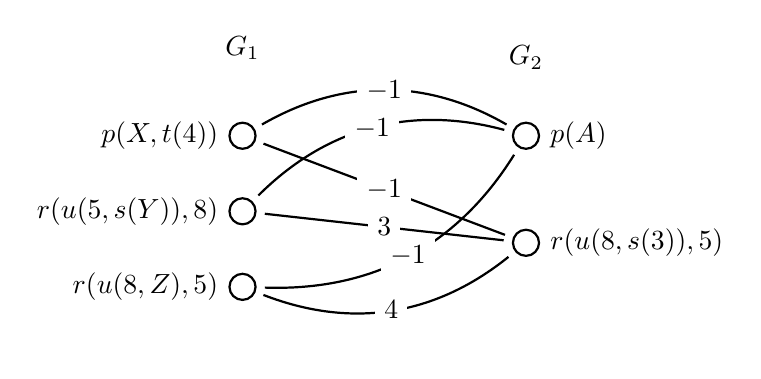
\begin{tikzpicture}[thick,
	fsnode/.style={draw, circle},
	ssnode/.style={draw, circle},
	every fit/.style={ellipse,text width=3cm},
	-,shorten >= 3pt,shorten <= 3pt,
	]
	
	% the vertices of U
	\begin{scope}[start chain=going below,node distance=6mm]
	\node[fsnode,on chain] (g1) [label=left: {$p(X, t(4))$}] {};
	\node[fsnode,on chain] (g2) [label=left: {$r(u(5,s(Y)),8)$}] {};
	\node[fsnode,on chain] (g3) [label=left: {$r(u(8,Z),5)$}] {};
	\end{scope}
	
	% the vertices of V
	\begin{scope}[xshift=3.6cm,start chain=going below,node distance=10mm]
	\node[ssnode,on chain] (h1) [label=right: {$p(A)$}] {};
	\node[ssnode,on chain] (h2) [label=right: {$r(u(8,s(3)),5)$}] {};
	\end{scope}
	
	% the set U
	\node [black, fit=(g1) (g3),label=above:{$G_1$}] {};
	% the set V
	\node [black, fit=(h1) (h2),label=above:{$G_2$}] {};
	
	\path (g1) edge[bend left] node [fill=white] {$-1$} (h1);
	\path (g1) edge node [fill=white] {$-1$} (h2);
	
	\path (g2) edge[bend left] node [fill=white] {$-1$} (h1);
	\path (g2) edge node [fill=white] {$3$} (h2);
	
	\path (g3) edge[bend right] node [fill=white] {$-1$} (h1);
	\path (g3) edge[bend right] node [fill=white] {$4$} (h2);
	]	
	\end{tikzpicture}
	\caption{The bipartite graph for the assignment problem from Example~\ref{example-mwm}}
	\label{fig:mwm}
	
\end{figure}

%\begin{algorithm}[hbtp]
%	\caption{Computing an msg $G$ for goals $G_1$ and $G_2$ with relation $\leqslant$} 
%	\label{algo-rel-1-mwm}
%	\begin{algorithmic}
%		\State $G = \{\}$ 
%		\State $E = \{\}$
%		\For {each ($A_1 \in G_1$)}
%			\For {each ($A_2 \in G_2$)}
%				\State $s\gets$ $\score(A_1, A_2)$
%				\State $E \gets E \cup \{(A_1, A_2, \mbox{s})\}$
%			\EndFor
%		\EndFor
%		\State $H \gets \MWM(E)$
%		\For {each $(A_1,A_2,s) \in H$} 
%			\State $G\gets G\cup\au_\leqslant(A_1,A_2)$ 
%		\EndFor
%	\end{algorithmic}
%\end{algorithm}

\begin{theorem}\label{thm-sqsubseteq-msg}
	Let $G_1$ and $G_2$ be goals and $N = \underset{A\in G_1}{\max}\{|\allterms(A)|\}$. Then a $\sqsubseteq$-msg of $G_1$ and $G_2$ can be computed in $\mathcal{O}\big(|G_1|\cdot |G_2|\cdot N +max(|G_1|,|G_2|)^3\big)$.
\end{theorem}
%\begin{proof}
%	First note how the atomic anti-unifications and the weights of the associated bipartite graph's edges can be computed simultaneously, by working out $\dau_\sqsubseteq(A_1,A_2)$ for each possible couple $(A_1,A_2)$ in $G_1\times G_2$ and keeping account of the number of non-variable terms encountered during the operation (or $-1$). Given that $\dau_\sqsubseteq(A_1,A_2)$ can obviously operate linearly in the number of terms appearing in $A_1$ (denoted $N$), the computation of all weights is carried out in a time not exceeding $\mathcal{O}(|G_1|.|G_2|.N)$.
%	
%	Now the obtained assignment problem can be solved by existing algorithms (such as the Hungarian method~\cite{assignment}) that compute a MWM in $\mathcal{O}(n^3)$, where $n$ is the number of vertexes appearing on the side of the bipartite graph that has the most vertexes. In our case, there are $|G_1|$ left vertexes and $|G_2|$ right vertexes so that a MWM algorithm can be ran in $\mathcal{O}(max(|G_1|,|G_2|)^3)$.
%\end{proof}

Note that the process described above finds \textit{a} $\sqsubseteq$-msg but there is no guarantee regarding \textit{which} $\sqsubseteq$-msg is found: as previously observed, the maximal $\terms$-value can sometimes be reached through different atomic structures. Another inconstant parameter from one msg to the other is the number of \textit{different} variables that are introduced in the generalization process. In fact, both aspects can sometimes be related, for example when minimizing the number of variables leads to the choice of a certain msg structure over another. A $\sqsubseteq$-most specific generalization that has \textit{as few} different variables as possible is often seen as an even more specific generalization; the computation of such a msg is the main topic of the following section.
%However, notice that invariably, all $\sqsubseteq$-msg's of two goals $G_1$ and $G_2$ only differ in their variable names, i.e. two $\sqsubseteq$-msg's necessarily harbor the same atomic structure, due to the matching process by essence trying to match in priority the atoms that have the heaviest structure.
	
	%%%%%%%%%%%%%%%%%%%%%%%%%%%%%%%%%%%%%%%%%%%%%%%%%%%
	%%%%%%%%%%%%%%%%%%%%%%%%%%%%%%%%%%%%%%%% 
	%%%%%%%%%%%%%%%%%%%%%%%%%%%%%%%%%%%%%%%%%%%%%%%%%%%
	\section{Dataflow Optimization}\label{section-relation-2}

Relations $\sqsubseteq$ and $\preceq$ are defined over substitutions that do not necessarily need to be \textit{injective}. Indeed, a single term occurring multiple times in one of the goals can potentially be generalized by two (or more) different variables. Therefore, some most specific generalizations may contain more different variables than others depending on the underlying variabilization process. 
Among two common generalizations of the same pair of goals, the common generalization that has more variables than the other can be considered \textit{less specific} as some information -- namely the fact that two or more values, possibly in different atoms, are equal -- has been abstracted by introducing different variables. In what follows, we will call the search of a common generalization with as few different variables as possible \textit{dataflow optimization}. The following example illustrates the concept over the finite domain from~\cite{clpbfd}. 

\begin{example}\label{ex:dataflow-bools}
	Consider the domain of Booleans $\mathbb{B} = \{true, false\}$ as well as the following goals: $G_1 = \{=\!\!(X, or(Y, Z)), =\!\!(V, and(Y, Z))\}$ and $G_2 = \{=\!\!(B, or(C, D)), =\!\!(A, and(C, D)), =\!\!(E, and(F, G))\}$. 
	Note that in $G_1$ the \textit{or} and \textit{and} operations are evaluated on the same values, represented by the multiple occurrences of the variables $Y$ and $Z$. In $G_2$ the \textit{or} and the \textit{and} operation from the second atom exhibit this very same behavior (represented by the variables $C$ and $D$), whereas the third atom represent an \textit{and} operation on different values. 
	Computing a $\preceq$-msg (and in this example, a $\sqsubseteq$-msg) for $G_1$ and $G_2$ can lead to two different generalizations, namely
	\[
	\begin{array}{lll}
	G & = & \{=\!\!(\Phi(X,B), or(\Phi(Y,C), \Phi(Z,D))), =\!\!(\Phi(V, E), and(\Phi(Y, F), \Phi(Z,G)))\}\\ %\\ = \{=\!\!(V_1, or(V_2, V_3)), =\!\!(V_5, and(V_6, V_7))\}
	G' & = & \{=\!\!(\Phi(X,B), or(\Phi(Y,C), \Phi(Z,D))), =\!\!(\Phi(V, A), and(\Phi(Y, C), \Phi(Z,D)))\}%= \{=\!\!(V_1, or(V_2, V_3)), =\!\!(V_4, and(V_2, V_3))\}\\
	\end{array}
	\] 
	Clearly, both generalizations are correct msg's, but the fact that all the variables in $G$ only occur once merely denotes that there exist six variables that together can make $G$ true. The repetition of $Y$ and $Z$ in $G_1$ as well as their connection with $C$ and $D$ is a lost information, abstracted by the anti-unification process. On the other hand, $G'$ by harboring less different variables introduces less variable abstraction, effectively depicting some dataflow logic that is common to $G_1$ and $G_2$, through the occurrence of $\Phi(Y,C)$ and $\Phi(Z,D)$ in both its atoms. On that level, $G'$ can be considered less general than $G$. 
\end{example}

Dataflow optimization thus formally boils down to finding, among a group of common generalizations for two goals $G_1$ and $G_2$, a goal $G$ such that $|\vars(G)|$ is minimal. In Example~\ref{ex:dataflow-bools}, we were interested in finding, among all possible msg's of $G_1$ and $G_2$, one that harbors a minimal number of variables; it makes sense, since abstracting one Boolean value with two different variables can be too liberal, depending on the applications. In that case of dataflow optimization, where the target goal must be a msg (i.e. when both structure and dataflow must be optimized), the dataflow problem is NP-complete. The same is true for lcg's. In order to show this formally, we consider a formulation in terms of decision problems.

%is a straightforward concern given that capturing as much common dataflow structure amongst $G_1$ and $G_2$ can further improve a msg's specificity and thus quality. 
\begin{theorem}\label{thm-dataflow-np-complete}
	Let MSG-MIN (resp. LCG-MIN) denote the following decision problem: "Given goals $G_1$, $G_2$ and a constant $p\in \mathbb{N}_0$, does there exist a $\leqslant$-msg (resp. $\leqslant$-lcg) of $G_1$ and $G_2$ that has less than $p$ different variables?". MSG-MIN and LCG-MIN are NP-complete.
\end{theorem}
%\begin{proof}
%	First, let us consider MSG-MIN. It clearly belongs to NP. Indeed, given an arbitrary generalization $G$, we can verify in polynomial time whether it is a most specific generalization. The procedure is as follows. We can compute at least one $\leqslant$-msg, say $G'$, in polynomial time (see Theorem~\ref{thm-preceq-lcg} for relation $\preceq$ and Theorem~\ref{thm-sqsubseteq-msg} for relation $\sqsubseteq$). It suffices then to compare the $\tau$-value of $G'$ with that of $G$ in order to decide whether $G$ is a msg. Next, verifying whether the number of variables in $G$ is bounded by a constant is obviously achieved in polynomial time as well.
%	
%	In order to prove NP-hardness, we will construct a reduction from the well-known set cover problem (known to be NP-complete~\cite{karp}) to MSG-MIN. The set cover problem in its decision-problem version (denoted SCP), can be formulated as follows. Given a constant $p \in \mathbb{N}_0$, a universe $U$ of values and a collection $S$ composed of $n$ sets $\{S_1, \dots, S_n\}$ that cover $U$, i.e. $U = \underset{i=1}{\overset{n}{\cup}}S_i$, the problem is to decide whether there exists $p$ subsets from $S$ that still cover $U$.
%	
%	We can transform an arbitrary instance of SCP into MSG-MIN as follows. Let us consider without loss of generality a universe $U$ where the elements are lowercase strings and $p \in \mathbb{N}_0$ a constant. Given a collection of sets $S=\{S_1, \dots, S_n\}$ we construct an instance of MSG-MIN as follows. In our construction we use $n+1$ different variables, namely $V$ and $(W_i)_{i\in1..n}$. We use $x_j$ to denote some element of $U$; these elements being strings, we can easily use them as predicate names. The construction of goals $G_1$ and $G_2$ proceeds then as follows:
%	
%	\begin{algorithmic}
%		\State $G_1 = \{\}$ 
%		\State $G_2 = \{\}$ 
%		\For {each ($S_i \in S$)}
%		\For {each ($x_j \in S_i$)}
%		\State $G_1 \gets G_1\cup \{x_j(V)\}$				
%		\State $G_2 \gets G_2\cup \{x_j(W_i)\}$
%		\EndFor
%		\EndFor
%	\end{algorithmic}
%	Note that all the atoms in $G_1$ have the same argument (namely the variable $V$) and there are as many atoms in $G_1$ as there are distinct elements in $S$. In $G_2$, however, there is an atom of the form $x_j(W_i)$ for each element $x_j$ occurring in $S_i$.
%	
%	The construction is such that any $\leqslant$-msg of $G_1$ and $G_2$ will be a version of $G_1$ where each occurrence of a variable $V$ is replaced by $\Phi(V, W_k)$ for some $W_k\in\vars(G_2)$ (where $\Phi$ is a variabilization function). Now, introducing such a variable $\Phi(V, W_k)$ in the generalization will allow to reuse the same variable for all the atoms $x_j(V)$ in $G_1$ that have a corresponding $x_j(W_k)$ in $G_2$. In other words, choosing to have variable $\Phi(V,W_k)$ in the $\leqslant$-msg is the same as selecting the subset $S_k$ to be part of the solution of the set cover problem. Consequently, using this transformation MSG-MIN can be used to decide SCP. Since the transformation can clearly be done in polynomial time, and since SCP is known to be NP-complete, we conclude that MSG-MIN is NP-complete as well.
%	
%	Now let us prove the result for LCG-MIN. We know that a $\leqslant$-lcg can be computed in polynomial time, so that a positive instance of LCG-MIN can be verified just like it can be for MSG-MIN. Moreover, the absence of non-variable terms in the transformation from SCP to MSG-MIN above allows us to reuse said transformation as-is to prove that LCG-MIN is NP-hard. Indeed, since the obtained anti-unification problem doesn't harbor terms other than variables, it is both an instance of MSG-MIN and LCG-MIN. LCG-MIN is therefore also NP-complete.
%\end{proof}

%Note that Theorem~\ref{thm-dataflow-np-complete} effectively concerns the NP-completeness of the statement for three common generalization patterns: $\sqsubseteq$-msg, $\preceq$-msg and $\preceq$-lcg -- the two latter being one and the same concept. The proof can in fact be adapted straightforwardly to the last of our subcases, namely the largest common generalization with relation $\sqsubseteq$. This observation is formalized in the following corollary.
%\begin{corollary} 
%	Let $G_1$ and $G_2$ be goals, and $p\in\mathbb{N}_0$ some constant. The decision problem ``does there exist a $\leqslant$-lcg of $G_1$ and $G_2$ that has less than $p$ different variables?'' is NP-complete. 
%\end{corollary} 
%\begin{proof}
%	The proof is analogous to that of Theorem~\ref{thm-dataflow-np-complete}. 
%	A generalization $G$ of two goals $G_1$ and $G_2$ can be verified to be a $\leqslant$-lcg by computing such a lcg (which can be done in a polynomial time), comparing their lengths and counting the number of variables in $G$. 
%	
%	Next, the reduction from SCP exposed above can be used as-is, since the obtained anti-unification instance harbors no term at all, so that in this case any generalization is a $\leqslant$-lcg iff it is a $\leqslant$-msg.
%\end{proof}
Now instead of looking to \textit{minimize} the number of different variables in the computed generalization $G$, one could be interested in \textit{forcing} to preserve all the dataflow implied in the generalized goals, not allowing to abstract away the links that appear in the goals' terms. Intuitively, this can be done by forbidding any term from one of the input goals to have more than one "corresponding term" in the other input goal. In other words, the dataflow is considered entirely preserved if the underlying variabilization function $\Phi$ doesn't associate any term with two or more different terms at the same time. Formally, this amounts to using an \textit{injective version} of our generalization relations. We say that a generalization relation is injective if its definition only holds for injective substitutions. For a common generalization $G$ of goals $G_1$ and $G_2$ and for some function $\Phi$ associating fresh variable names to couples of variables, this implies when using an anti-unification algorithm (e.g. Algorithm~\ref{algo-rel-1-lcg}) that for any two different variables $\Phi(T_1, T_2)$ and $\Phi(T_3, T_4)$ appearing in $G$, it holds that $T_1 \neq T_3 \neq T_2 \neq T_4\neq T_1$. We will denote by $\sqsubseteq^\iota$ (resp. $\preceq^\iota$) the versions of $\sqsubseteq$ (resp. $\preceq$) that exhibit this property.

\begin{example}
    Consider the injective relation $\preceq^\iota$ as well as the goals 
    	$G_1 = \{and(A,B), or(B,C), xor(C,A)\}$ and
    	$G_2 = \{and(X,Z), or(Y,X), xor(Z,Y)\}$.
    The only common generalizations are $\emptyset$, $\{and(\Phi(A,X),\Phi(B,Z))\}, \{or(\Phi(B,Y), \Phi(C,X))\}$ and $\{xor(\Phi(C,Z), \Phi(A,Y))\}$. No common generalization of size larger than 1 exists, since (at least) one of the matching substitutions is not injective. For example, the goal $G = \{and(\Phi(A,X), \Phi(B,Z)), or(\Phi(B,Y), \Phi(C,X))\}$ is not a common generalization of $G_1$ and $G_2$, since (at least) one of the substitutions mapping this goal to $G_1$ or $G_2$ is not injective. Indeed, the substitution $[\Phi(A,X) \mapsto A, \Phi(B,Z) \mapsto B, \Phi(B,Y) \mapsto B, \Phi(C,X) \mapsto C]$ maps both $\Phi(B,Z)$ and $\Phi(B,Y)$ to $B$; this is sufficient to reach the conclusion that $G$ is not an injective generalization of $G_1$ and $G_2$. Note that in this case, the other potential substitution, i.e. the one mapping $G$ on $G_2$, is not injective either. 
\end{example}

The two following observations immediately result from the injective relations being more constrained versions of their non-injective counterparts. 

\begin{proposition}
	Relations $\sqsubseteq^\iota$ and $\preceq^\iota$ are quasi-orders. 
\end{proposition}

\begin{proposition}
	Let $G_1$ and $G_2$ be goals. If $G_1\sqsubseteq_\theta^\iota G_2$, then $G_1\sqsubseteq_\theta G_2$. If $G_1\preceq^\iota_\theta G_2$, then $G_1\preceq_\theta G_2$ and $G_1\sqsubseteq^\iota_\theta G_2$.
\end{proposition}

With an injective generalization relation, the computing of a msg is fundamentally dissociated from that of an lcg, as an msg is not necessarily a lcg due to the injectivity constraint. However, both situations are intractable. In order to show this formally, we define the following decision problem variant.

\begin{theorem}\label{thm-inj-np-complete}
	Let INJ denote the following decision problem: "Given an injective generalization relation $\leqslant^\iota$ along with goals $G_1$ and $G_2$ such that $|G_1|\le|G_2|$, verify whether there exists an ad hoc injective substitution $\theta$ such that $G_1\theta\subseteq G_2$". INJ is NP-complete.
\end{theorem}
%\begin{proof}
%	INJ is in NP: given a relation $\leqslant^\iota$, goals $G_1$ and $G_2$ and a substitution (or renaming) $\theta$, it is possible to verify in polynomial time whether the application of $\theta$ on $G_1$ results on a subset of $G_2$ or not.
%	As for the proof of NP-hardness, we refer to~\cite{gen} in which the problem ``is $G_1$ a $\preceq^\iota$-lcg of $G_1$ and $G_2$?'' has been proved to be NP-complete using a polynomial reduction from the Induced Subgraph Isomorphism Problem~\cite{SYSLO198291}. The same reduction can be used for the other cases, leading to the conclusion that INJ is NP-complete.
%\end{proof}

INJ is basically the verification of whether a goal $G_1$ can be adequately mapped onto (a subset of) another goal $G_2$. If there exists a substitution $\theta$ (resp. a renaming $\rho$) making this possible, then $G_1$ is a $\sqsubseteq^\iota$- (resp. $\preceq^\iota$-)largest \textit{and} most specific generalization of $G_1$ and $G_2$, since no larger nor structurally more specific goal than $G_1$ can exist for this specific situation.

Due to the inherent intractability of injective relations, it is sometimes preferable to make use of tractable abstractions rather than exact brute-force algorithms, especially if a quick and approximate (though entirely dataflow-preserving) anti-unification result suffices for the application at hand. In the next section, we give such an efficient -- yet highly accurate~-- abstraction for the computation of $\preceq^\iota$-lcg's. 

	
	%%%%%%%%%%%%%%%%%%%%%%%%%%%%%%%%%%%%%%%%%%%%%%%%%%%
	%%%%%%%%%%%%%%%%%%%%%%%%%%%%%%%%%%%%%%%% 
	%%%%%%%%%%%%%%%%%%%%%%%%%%%%%%%%%%%%%%%%%%%%%%%%%%%
	\section{The $k$-swap Stability Abstraction}\label{section-relation-3}
In what follows, we introduce an abstraction for the largest common generalization with respect to $\preceq^\iota$ that can be computed in polynomial time. The abstraction was already introduced in~\cite{gen} but no formal proof of its complexity was given. The abstraction is based on the \textit{$k$-swap stability} property, which is in turn defined in terms of \textit{pairing generalizations}. 

\begin{definition}
	Let $G_1$ and $G_2$ be two renamed apart goals and $G$ be a $\preceq^\iota$-common generalization of $G_1$ and $G_2$ such that $G\subseteq G_1$. Let $\rho$ be any renaming such that $G\rho\subseteq G_2$. The \emph{pairing generalization} of $G$, denoted $\pi(G)$, is the set of pairs $(A_1, A_2) \in G_1\times G_2$ such that $\forall(A_1, A_2)\in\pi(G):A_1\rho = A_2$. 
\end{definition}

\begin{example}
	Considering the goals $G_1 = \{p(A), p(B), q(A)\}$ and $G_2 = \{p(X), q(Y)\}$, it is easy to see that $G = \{p(\Phi(B,X)), q(\Phi(A,Y))\}$ is a $\preceq^\iota$-common generalization of them. The corresponding pairing generalization is $\pi(G) = \{(p(B), p(X)), (q(A), q(Y))\}$.
\end{example} 

The notion of a pairing generalization renders thus explicit the corresponding atoms from the generalized goals that contribute to the generalization.
As a slight abuse of language, given a pairing generalization $\pi$ of some generalization $G$ for goals $G_1$ and $G_2$, we will simply say that $\pi$ is a \textit{pairing for $G_1$ and $G_2$}. 
Pairings can be used to express a notion of goal \textit{stability} in the following sense.

\begin{definition}\label{def-k-swap-stable}
	Let $G_1$ and $G_2$ be two renamed apart goals and $G$ be a $\preceq^\iota$-common generalization of $G_1$ and $G_2$ such that $G\subseteq G_1$. $G$ is \emph{k-swap stable} if and only if there does not exist some generalizations $\hat{G}$ and $G'$ of $G_1$ and $G_2$ such that $\hat{G}\supset G'$ and $|\pi(G)\cap\pi(G')|\ge |\pi(G)|-k$ for some $k\in\mathtt{N}$.
\end{definition}

Intuitively, a generalization $G$ is $k$-swap stable if it is impossible to transform $G$ into a larger generalization $\hat{G}$ in spite of ``swapping'' at most $k$ pairs in $\pi(G)$.
%Intuitively, a generalization $G$ is $k$-swap stable if ``swapping'' at most $k$ pairs in $\pi(G)$ -- i.e. removing pairs or replacing them with other pairs in $G_1\times G_2$ -- would not make $G$ easily extensible into some greater generalization $\hat{G}$. 
%Put differently, $G$ is \textit{not} $k$-swap stable if $k$ editions, or swaps, in $\pi(G)$ suffice to consequently extend $G$ into some other common generalization $\hat{G}$. 
This stability notion gives a characterization of the quality of a computed generalization. If a generalization is 0-swap stable (the weakest characterization), it cannot be extended by adding another atom but this guarantees in no way that a larger generalization could not be found. If a generalization $G$ is $k$-swap stable (for $k>0$), it means that even if we exchange up to $k$ pairs in $\pi(G)$ by others, the generalization cannot be extended into a larger one. Consequently, if a generalization is $k$-swap stable for $k$ the number of atoms in the smallest of the two goals (denoted by $\infty$-swap stable), it means that the computed generalization is a largest common generalization. 
%
Operationally, when naively searching for a lcg by backtracking, the fact that a computed generalization is $k$-swap stable means that one should backtrack by \textit{more} than $k$ choice points in order have a chance of finding a larger generalization. 

%Operationally, each swap can be seen as a possible backtracking in a naive algorithm trying to compute a $\preceq^\iota$-lcg. When computing a 0-swap stable generalization
%Indeed, when $k$ grows, the outputted generalization gets higher accuracy as it reconsiders more choices that were made during the construction of $G$. If $k = \infty$, building a generalization through $k$-swaps will perform an exhaustive search, as all choices that are made will be reconsidered. 

\begin{example}\label{ex:k-swap-stable}
   	Consider the goals $G_1 = \{add(X,Y,Z), even(X), odd(Z), p(Z)\}$ and $
G_2 = \{add(A,B,C), add(C,B,A), even(C), odd(A), p(C)\}$. 
   	 $\pi_1= \{(add(X,Y,Z), add(A,B,C))\}$ is not $0$-swap stable. Indeed, we can enlarge $\pi_1$ by adding $(p(Z),p(C))$, in order to obtain 
   	$\pi_2 = \{(add(X,Y,Z),add(A,B,C)), (p(Z),p(C))\}.$
   	Note that $\pi_2$ is $0$-swap stable, it is impossible to add another pair to $\pi_2$ and still obtain a common generalization. 
   	It is also $1$-swap stable, seeing that replacing (or removing) one of the pairs doesn't lead to a pairing readily extensible to a pairing of size strictly greater than~$2$. However, $\pi_2$ is not $2$-swap stable. Indeed, replacing the pair $(add(X,Y,Z),add(A,B,C))$ by the pair $(add(X,Y,Z), add(C,B,A))$ in $\pi_2$ and removing the now incompatible pair $(prime(Z),prime(C))$ (i.e. choosing the renaming $[X\mapsto C, Y\mapsto B, Z\mapsto A]$ instead of $[X\mapsto A, Y\mapsto B, Z\mapsto C]$) gives rise to $\pi_2' = \{(add(X,Y,Z),add(C,B,A))$, which can readily be extended into
   	   		$\pi_3 = \{(add(X,Y,Z),add(C,B,A)), (even(X),even(C)), (odd(Z),odd(A))\}$
   	which is a pairing of size 3. The latter being $\infty$-swap stable, it represents a $\preceq^\iota$-lcg, namely
   		$\hat{G} = \{add(\Phi(X,C), \Phi(Y,B), \Phi(Z,A)), even(\Phi(X,C)), odd(\Phi(Z,A))\}$
\end{example}
An algorithm has been introduced in~\cite{gen} that builds up a $k$-swap stable generalization using the process suggested in Example~\ref{ex:k-swap-stable}. Its practical performance has been assessed on different test cases. The tests indicate that the $k$-swap stability property represents a well-suited approximation of the concept of $\preceq^\iota$-lcg. Indeed, in all test cases the size of the $k$-swap stable generalization was at least $90\%$ of the size of an lcg for the same anti-unification problem, while the computational time was radically reduced -- especially as the size of the input goals grows\footnote{For example, with $k$ fixed to 4, anti-unifying goals harboring 15 to 22 atoms, each of arity between 1 and 3, comes on average down from more than 7 minutes (using bruteforce) to 272 milliseconds (using the algorithms presented in this section), while the size of the computed generalization is on average $95\%$ of the size of a lcg. More detailed test results are exposed in~\cite{gen}.}. However, in~\cite{gen} only pragmatical aspects have been explored; the theoretical foundations of the $k$-swap technique were not detailed, and  no actual time complexity upper bound has been demonstrated. We fill this gap in the remainder of this section. First, we introduce the algorithm, then we formally prove that its time complexity is polynomially bounded. Before introducing the algorithm, which is essentially composed of two sub-algorithms, we give some notations that will facilitate their formulation. First, we define an operator that allows to combine two pairings into a single pairing.
	
\begin{definition}
	Let $G_1$ and $G_2$ be two renamed apart goals. The \emph{enforcement operator} is defined as the function $\enforce: (G_1\times G_2)^2 \mapsto (G_1\times G_2)$ such that for two pairing generalizations $\pi$ and $\pi'$ for $G_1$ and $G_2$, $\pi \enforce \pi' = \pi' \cup M$ where $M$ is the largest subset of $\pi$ such that $\pi'\cup M$ represents a $\preceq^\iota$-common generalization of $G_1$ and $G_2$. 
\end{definition}
	
In other words, $\pi\enforce\pi'$ is the mapping obtained from $\pi\cup\pi'$ by eliminating those pairs of atoms $(A,A')$ from $\pi$ that are \textit{incompatible} with some $(B,B')\in\pi'$ either because they concern the same atom(s) or because the involved renamings cannot be combined into a single injective renaming. 
	
\begin{example}
	Consider 
	$\pi = \{(p(X, Y), p(A, B)), (q(X), q(A))\}$ as a pairing for two goals $G_1$ and $G_2$. Suppose $\pi' = \{(r(Y), r(C))\}$ is also a pairing for $G_1$ and $G_2$. Enforcing $\pi'$ into $\pi$ gives $\pi\enforce\pi' = \{(q(X), q(A)), (r(Y), r(C))\}$. Indeed, this can be seen as forcing $Y$ to be mapped on $C$; therefore the resulting pairing generalization can no longer contain $(p(X, Y), p(A, B))$ as the latter maps $Y$ on $B$. 
\end{example}

For $\pi_1$ and $\pi_2$ pairings we will also denote by $\compatible_{\pi_1}(\pi_2)$ the subset of $\pi_2$ of which each element can be added to $\pi_1$ such that the result is a pairing (i.e. there is no injectivity conflict in the associated renaming). Finally, we use $\gen(G_1, G_2)$ to represent those atoms from $G_1$ and $G_2$ that are variants of each other, formally $\gen(G_1,G_2)=\{(A,A')\:|\:A\in G_1, A'\in G_2\mbox{ and }A\rho=A'\mbox{ for some renaming }\rho\}$. 
%
The first algorithm is depicted in Algorithm~\ref{alg:kswap}. The algorithm represents the construction of a $k$-swap stable generalization of goals $G_1$ and $G_2$. At each round, the process tries to transform the current generalization $\pi$ (which initially is empty) into a larger generalization by forcing a new pair of atoms $(A,A')$ from $\gen(G_1,G_2)$ in $\pi$, which is only accepted if doing so requires to swap no more than $k$ elements in $\pi$. More precisely, the algorithm selects a subset of $\pi$ (namely $\pi_s$) that can be swapped with a subset $\pi_c$ of the remaining mappings from $\gen(G_1,G_2)\setminus\pi$ such that the result of replacing $\pi_s$ by $\pi_c$ in $\pi$ and adding $(A,A')$ constitutes a pairing. Note how condition 1 in the algorithm expresses that $\pi_s$ must include at least those elements from $\pi$ that are not compatible with $(A,A')$.
The search continues until no such $(A,A')$ can be added.

\begin{algorithm}[hbtp]
	\caption{Computing a $k$-swap stable generalization $G$ for goals $G_1$ and $G_2$}
	\label{alg:kswap}
	\begin{algorithmic}
		\State $\pi\gets\emptyset$
		\Repeat
			\State $found\gets false$
			\ForAll{$(A,A')$ in $\gen(G_1, G_2)\setminus \pi$}
				\State select $\pi_s \subseteq \pi$ and $\pi_c\subseteq \gen(G_1, G_2)\setminus(\pi \cup\{(A,A')\})$ such that:
				\State \hspace*{3ex}(1) $\pi_s\supseteq \pi\setminus \pi\enforce\{(A,A')\}$
				\State \hspace*{3ex}(2) $|\pi_s| \le k$
				\State \hspace*{3ex}(3) $|\pi_c| = |\pi_s|$
				\State \hspace*{3ex}(4) $\pi\setminus \pi_s\cup \pi_c\cup\{A,A'\}$ is a pairing generalization of $G_1$ and $G_2$
				
				\If{such $\pi_c$ and $\pi_s$ are found}
					\State $\pi\gets \pi\setminus \pi_s\cup \pi_c \cup \{(A,A')\}$
					\State $found\gets true$
					\State \textbf{break} out of the \textbf{for} loop
				\EndIf
			\EndFor
		\Until $\neg found$
		\State $G \gets \dom(\pi)$
	\end{algorithmic}
\end{algorithm}	

The main operation of Algorithm~\ref{alg:kswap}, namely the selection of $\pi_s$ and $\pi_c$, is detailed in Algorithm~\ref{alg:selection} which aims to select the parts of the pairings to be swapped in order to enlarge the resulting pairing under construction ($\pi$) by the couple $(A,A')$.
To that purpose $\pi_s$ is initialized with the part of $\pi$ that is incompatible with the pair of atoms $(A,A')$ that we wish to enforce into the generalization. Its replacement mapping $\pi_c$ is initially empty and the algorithm subsequently searches to construct a sufficiently large $\pi_c$ (the inner while loop). During this search, $S$ represents the set of candidates, i.e. couples from $\gen(G_1,G_2)$ that are not (yet) associated to the generalization. In order to explore different possibilities with backtracking, the while loop manipulates a stack $GS$ that records alternatives for $\pi_c$ with the corresponding set $S$ for further exploration. 
\begin{algorithm}[hbtp]
\caption{Selecting $\pi_s$ and $\pi_c$ for a given $(A,A')$}
\label{alg:selection}
	\begin{algorithmic}
		\State $GS \gets \{\}$,  $BS \gets \{\}, \pi_c \gets\{\}$
		\State $\pi_s \gets \pi\setminus\pi\enforce\{(A,A')\}$
		\State $S \gets \gen(G_1, G_2) \setminus\pi\enforce\{(A,A')\}$
		\While{$|\pi_c| < |\pi_s| \mbox{ and } |\pi_s|\le k$}
			\While{$|\pi_c| < |\pi_s| \mbox{ and } \neg (\compatible_{\pi\setminus\pi_s\cup\pi_c}(S) = \{\} \mbox{ and } GS = \{\})$}
				\ForAll{$p$ in $\compatible_{\pi\setminus\pi_s\cup\pi_c}(S)$}	
					\State $push(GS, (\pi_c\cup p, S\setminus\{p\}))$
				\EndFor
				\State $(\pi_c, S)\gets pop(GS)$
			\EndWhile
			\If{$|\pi_c|<|\pi_s|$}
				\ForAll{$p$ in $\pi\setminus\pi_s$}
					\State $enter(BS, \pi_s\cup\{p\})$
				\EndFor
				\If{$BS\neq\{\}$}
					\State $\pi_s\gets exit(BS)$
					\State $\pi_c\gets\{\}$
					\State $S\gets \gen(G_1, G_2)\setminus(\pi\cup \{(A,A')\})$
				\Else
					\State \textbf{return} $\bot$
				\EndIf
			\EndIf
		\EndWhile
		\If{$|\pi_c|=|\pi_s|$}
			\State \textbf{return} $\pi_s, \pi_c$
		\EndIf
			\State r\textbf{return} $\bot$
	\end{algorithmic}
\end{algorithm}

If the search for $\pi_c$ was without a satisfying result (i.e. no $\pi_c$ is found equal in size to $\pi_s$), the algorithm continues by removing another couple from $\pi$ (thereby effectively enlarging $\pi_s$). The rationale behind this action is that there might be a couple in $\pi$ that is ``blocking'' the couples in $S$ from addition to $\pi$. In order to achieve the removal of such potentially blocking couples, an arbitrary couple from $\pi\setminus\pi_s$ is selected, and alternatives are recorded in a queue ($BS$). Note the use of a queue (and its associated operations \textit{enter} and \textit{exit}) as opposed to the stack $GS$.
%
The process is repeated until either $|\pi_c|=|\pi_s|$ in what case we have found a suitable $k$-swap, or until $|\pi_s|>k$ in what case we have not, and the algorithm returns $\bot$. %Note how Algorithm~\ref{alg:selection} behaves analogously to an $A*$ search.

While the algorithms have been proven to correctly compute a $k$-swap stable generalization~\cite{gen}, no result on their complexity has yet been formally established. 

\begin{theorem}\label{thm-k-swap-stable}
	For a given and constant value of $k$, the combination of Algorithms~\ref{alg:kswap} and~\ref{alg:selection} computes a $k$-swap stable common generalization of input goals $G_1$ and $G_2$ in polynomial time $\mathcal{O}((\alpha M)^{k+1})$, with $0 \le M \le |gen(G_1, G_2)|$ and $0 \le \alpha \le \textit{min}(|G_1|,|G_2|)$.
\end{theorem}
\begin{proof}
	In order to search for a suited $\pi_c$ to be swapped with a certain $\pi_s$, Algorithm~\ref{alg:selection} must try to add $|\pi_s|$ couples to $\pi\setminus\pi_s$ among the couples in $S$ that are compatible with it. To simplify notation, let $i = |\pi_s|$ and $n = |\compatible_{\pi\setminus\pi_s\cup\pi_c}(S)|$. Note that at any moment $i \le k$. The attempt of Algorithm~\ref{alg:selection} to find $\pi_c$ is essentially a search of a combination of $i$ couples among $n$; that is $\binom{n}{i}$ possibilities to explore. We have $\binom{n}{i} = \frac{n!}{i!(n-i)!}$ which reduces to a polynomial of degree $n^i$:
	\begin{gather*}
	\begin{array}{lll}
	\frac{n!}{i!(n-i)!} &=& \frac{n\cdot (n-1)\dots\cdot (n-(i+1) \cdot (n-i)\cdot (n-(i-1))\cdot\dots\cdot 1}{i!\cdot(n-i)\cdot (n-(i-1))\cdot\dots\cdot 1}
	= \frac{n\cdot (n-1)\dots\cdot (n-(i+1))}{i!}
	\approx \mathcal{O}(n^i)
	\end{array}
	\end{gather*}
	
	If no suiting $\pi_c$ is found during such a search, 
	%Algorithm~\ref{alg:selection} retries for all other potential $\pi_s$ pairings. If still no $\pi_c$ is found, 	
	then $\pi_s$ gets enlarged, having its size $m$ increased by (at least) one unit.
	%
	In the worst case, the size $i$ of $\pi_s$ is, at the start of Algorithm~\ref{alg:selection}, equal to $1$. It then gets incremented by one, until it reaches $k$ (each time more atoms from $\pi$ being considered to be part of $\pi_s$). 
	%
	Let $p$ denote the size of the pairing $\pi$ under construction, that is $p = |\pi|$. As $k$ is constant, if  backtracking is exhaustive there are $\sum\limits_{i=1}^{k} \binom{p}{i}$
%	\begin{gather*}
%	\begin{array}{lll}
%	\sum\limits_{i=1}^{k} \binom{p}{i} &=& \sum\limits_{i=1}^{k} \mathcal{O}(p^i) \\ &=& \mathcal{O}(p) + \mathcal{O}(p^2) + ... \mathcal{O}(p^k) \\
%	&=&  \mathcal{O}(p^k) 
%	\end{array}
%	\end{gather*}
	possibilities for $\pi_s$ pairings that are explored this way. Each of these $\pi_s$ pairings leads to the search for a corresponding $\pi_c$ pairing. As such, the overall search carried out by Algorithm~\ref{alg:selection} takes a number of iterations that is in the worst case represented by
	\[
	\begin{array}{lllll}
		\sum\limits_{i=1}^{k} \binom{p}{i}\cdot\binom{n}{i} & \approx & \sum\limits_{i=1}^{k} \mathcal{O}(p^i)\cdot\mathcal{O}(n^i) & \approx & \mathcal{O}((p\cdot n)^k)
	\end{array}
	\]
Given that $n$ is bound by the number of compatible couples of atoms from $G_1\times G_2$, we will denote the worst-case time complexity of Algorithm~\ref{alg:selection} by $\mathcal{O}((p\cdot M)^k)$ with $M \le |\gen(G_1,G_2)|$ and $p$ the length of the pairing under construction $\pi$.
		
%	\begin{gather*}
%	\begin{array}{lll}
%	\sum\limits_{i=1}^{k} p^i \cdot n^i&=&\sum\limits_{i=1}^{k} (p\cdot n)^i \\
%	&=& (p\cdot n) + (p\cdot n)^2 + (p\cdot n)^3 + \dots + (p\cdot n)^k  \\
%	&=& \mathcal{O}((p\cdot n)^k) \\
%	&=&  \mathcal{O}((p\cdot M)^{k}) \mbox{ with } M \le |\gen(G_1, G_2)|
%	\end{array}
%	\end{gather*}
%	\begin{gather*}
%	\begin{array}{lll}
%	\mathcal{O}(n^m) \cdot \mathcal{O}(p^k) &=& \mathcal{O}(M^{Mk}) \mbox{ with } M \le |\gen(G_1,G_2)|
%	\end{array}
%	\end{gather*}
	
	
	
	%The variable $n$ is majored by the total compatible couples $|\gen(G_1, G_2)|$, so that the overall search carried out by Algorithm~\ref{alg:selection} takes a number of iterations of amplitude
	% Note that $\pi$ being the pairing under construction, its size $p$ is majored by $\min(|G_1|,|G_2|)$. 
	
Turning our attention to Algorithm~\ref{alg:kswap} it is clear that the size of pairing $\pi$ is incremented by $1$ in each iteration of the \textit{repeat}-loop, since $found$ must be true for a new iteration to occur. As such, in the worst-case scenario there can be as many iterations as there are atoms in the smallest goal amongst $G_1$ and $G_2$, seeing that a generalization size cannot exceed that of the goals it generalizes. We will denote this number by $\alpha = \min(|G_1|, |G_2|)$.
%
As for the inner loop of Algorithm~\ref{alg:kswap}, it can browse through up to $|\gen(G_1, G_2)| - p$ candidates for choosing the couple $(A,A')$ that will be enforced in the pairing $\pi$. This gives us at most $
	%\begin{gather*}
	\begin{array}{lll}
	\sum\limits_{p=1}^{\alpha}(|\gen(G_1, G_2)| - p) &\approx &\sum\limits_{p=1}^{\alpha}\mathcal{O}(M - p)
	%\mathcal{O}(\min(|G_1|,|G_2|) \cdot |\gen(G_1,G_2)|) &=& \mathcal{O}(M^2) 	
	\end{array}
	$ %\end{gather*} 
	iterations of Algorithm~\ref{alg:kswap}.
%	Let us now focus on the search of the pairing $\pi_c$ to be swapped with $\pi_s$. At any moment there are as many potential couples to populate $\pi_c$ as there are pairs in the set $\compatible_{\pi\setminus\pi_s\cup\pi_c}(S)$. Let us denote by $l$ the maximal number of elements that this set beholds during the algorithm's execution, we have $l \le |\gen(G_1,G_2)|$. The search for a $\pi_c$ is then, similarly as for $\pi_s$ above, achieved in a time majored by $\binom{l}{k}$. For $\pi_c$ to suitably replace $\pi_s$ in $\pi$, there are indeed $k$ pairs to be chosen amongst all the potential compatible pairs in $S$ that are compatible with the version of $\pi$ under construction (namely $\pi\setminus\pi_s\cup\pi_c$). With a similar reasoning as above, this can be expressed as
%	\begin{gather*}
%	\sum\limits^{max}_{n=1}\binom{l}{k} = \sum\limits_{n=1}^{max}\mathcal{O}(l^k) = \mathcal{O}(l^{ck}) \mbox{ with } c \mbox{ a natural }
%	\end{gather*} 
	%$\mathcal{O}(M^{ck})$, where $c$ is a constant and $M$ is the maximal size of the set $\compatible_{\pi\setminus\pi_s\cup\pi_c}(S)$ during the algorithm's execution (this size being majored by $|gen(G_1,G_2)|$). 
	%The search of a $\pi_c$ being done for each considered $\pi_s$, the total complexity of Algorithm~\ref{alg:selection} can be expressed as the multiplication of both the complexities outlined above, i.e. $\mathcal{O}(max^{2k})\cdot \mathcal{O}(l^{ck})$. Because $l \le |\gen(G_1,G_2)|$ and $max\le max(|G_1|,|G_2|)$, both $l$ and $max$ are majored by $M = |G_1\times G_2|$, and the product can be written $\mathcal{O}(M^{(2+c)k}) = \mathcal{O}(M^{Ck})$ with $C$ a natural.
	%
	Algorithm~\ref{alg:selection} being called at each inner loop iteration of Algorithm~\ref{alg:kswap}, we can represent the time complexity of the combined algorithms by
	%\begin{gather*}
	%\begin{array}{lll}
	$\sum\limits_{p=1}^{\alpha}\mathcal{O}(M-p) \cdot \mathcal{O}((p\cdot M)^k) \approx \sum\limits_{p=1}^{\alpha} \left((M-p)\cdot p^k\cdot M^k\right)$
%\end{array}
%	\end{gather*}
	which can be rewritten as $
	M^{k+1}\cdot \left(\sum\limits_{p=1}^{\alpha} p^k\right) - M^k \cdot \left(\sum\limits_{p=1}^{\alpha} p^{k+1}\right)$.
	
	Since $\sum\limits_{p=1}^{\alpha} p^k \approx \mathcal{O}(\alpha^{k+1})$ and $\sum\limits_{p=1}^{\alpha} p^{k+1} \approx \mathcal{O}(\alpha^{k+2})$, we can conclude the total complexity to be of the order $\mathcal{O}((\alpha\cdot M)^{k+1}) - \mathcal{O}(\alpha^{k+2}\cdot M^k)$ which proves the result.
\end{proof}

Whenever there is a need to compute numerous anti-unifications of unordered goals with limited time resources, the $k$-swap stability abstraction allows to keep the search space tractable while outputting goals that are, on average, close in size to that of a lcg. Such situations can e.g. arise in static analysis techniques for large Horn clause programs, such as the assessment of structural similarity between algorithms expressed in CLP~\cite{clones}. 

%We have observed, through the implementation of a Prolog prototype built for the case of (unordered) Constraint Logic Programming goals, that Algorithms~\ref{alg:kswap} and~\ref{alg:selection} find a relatively good abstraction of a lcg (the outputted generalizations have 90\% to 100\% of a looked-upon lcg size in all our test cases) while significantly diminishing the amount of time required for finding such a common generalization (when each goal harbors 10 to 15 different variables and 15 to 20 atoms of arity between 1 and 3, the average execution of our test cases takes the execution time of 26 seconds with bruteforce mechanisms down to 91 milliseconds with the k-swap stability algorithm). Obviously the algorithm seems to run in polynomial time. 
	
	%%%%%%%%%%%%%%%%%%%%%%%%%%%%%%%%%%%%%%%%%%%%%%%%%%%
	%%%%%%%%%%%%%%%%%%%%%%%%%%%%%%%%%%%%%%%% Conclusion
	%%%%%%%%%%%%%%%%%%%%%%%%%%%%%%%%%%%%%%%%%%%%%%%%%%%
	\section{Conclusions and Future Work}\label{section-conclusion}
In this work, we have systematically studied different key notions and results concerning anti-unification of unordered goals, i.e. sets of atoms. We have defined different anti-unification operators and we have studied several desirable characteristics for a common generalization, namely optimal cardinality (lcg), highest $\tau$-value (msg) and variable dataflow optimizations. For each case we have provided detailed worst-case time complexity results and proofs. An interesting case arises when one wants to minimize the number of generalization variables or constrain the generalization relations so as they are built on injective substitutions. In both cases, computing a relevant generalization becomes an NP-complete problem, results that we have formally established.
In addition, we have proven that an interesting abstraction -- namely $k$-swap stability which was introduced in earlier work -- can be computed in polynomially bounded time, a result that was only conjectured in  earlier work. 

Our discussion of dataflow optimization in Section~\ref{section-relation-2} essentially corresponds to a reframing of what authors of related work sometimes call the \textit{merging} operation in rule-based anti-unification approaches as in~\cite{Baumgartner2017}. Indeed, if the "store" manipulated by these approaches contains two anti-unification problems with variables generalizing the same terms, then one can "merge" the two variables to produce their most specific generalization. If the merging is exhaustive, this technique results in a generalization with as few different variables as possible. In this work we isolated dataflow optimization from that specific use case and discussed it as an anti-unification problem in its own right.

While anti-unification of goals in logic programming is not in itself a new subject, to the best of our knowledge our work is the first systematic treatment of the problem in the case where the goals are not sequences but unordered sets. Our work is motivated by the need for a practical (i.e. tractable) generalization algorithm in this context. The current work provides the theoretical basis behind these abstractions, and our concept of $k$-swap stability is a first attempt that is worth exploring in work on clone detection such as~\cite{clones}. 

Other topics for further work include adapting the $k$-swap stable abstraction from the $\preceq^\iota$ relation to dealing with the $\sqsubseteq^\iota$ relation. 
A different yet related topic in need of further research is the question about what anti-unification relation is best suited for what applications. For example, in our own work centered around clone detection in Constraint Logic Programming, anti-unification is seen as a way to measure the distance amongst predicates in order to guide successive syntactic transformations. Which generalization relation is best suited to be applied at a given moment and whether this depends on the underlying constraint context remain open questions that we plan to investigate in the future. 

%The main results of this paper are the polynomial algorithms solving specific anti-unification problems, along with several worst-case time complexity results and proofs. 

% have made efforts to extend the classical anti-unification concepts to the case where the artefacts to generalize are unordered goals. We have done this by considering different levels of atomic abstraction through different generalization relations. W





%Throughout the paper, we have introduced four generalization relations. Figure~\ref{fig-interconnexion} shows how the four relations are linked on a conceptual level. $\sqsubseteq$ is the most general relation as generalization is defined with any substitution. Restricting the definition to injective substitutions or to renamings yields more specific relations, the intersection of which is relation $\preceq^\iota$ where variables are generalized through injective renamings. 

%\begin{figure}[htbp]
%	\begin{center}
%		\begin{tikzpicture}[x=0.75pt,y=0.75pt,yscale=-1,xscale=1]
%		%uncomment if require: \path (0,300); %set diagram left start at 0, and has height of 300
%		
%		%Shape: Ellipse [id:dp330479544492589] 
%		\draw   (150.05,144.64) .. controls (150.05,72.29) and (186.09,13.64) .. (230.55,13.64) .. controls (275,13.64) and (311.05,72.29) .. (311.05,144.64) .. controls (311.05,216.99) and (275,275.64) .. (230.55,275.64) .. controls (186.09,275.64) and (150.05,216.99) .. (150.05,144.64) -- cycle ;
%		%Shape: Ellipse [id:dp3140532351606715] 
%		\draw   (165,87.62) .. controls (165,64.99) and (193.75,46.64) .. (229.22,46.64) .. controls (264.69,46.64) and (293.45,64.99) .. (293.45,87.62) .. controls (293.45,110.26) and (264.69,128.61) .. (229.22,128.61) .. controls (193.75,128.61) and (165,110.26) .. (165,87.62) -- cycle ;
%		%Shape: Ellipse [id:dp9580468020324391] 
%		\draw   (261.25,53.46) .. controls (285.77,54.29) and (304.38,90.37) .. (302.81,134.06) .. controls (301.24,177.74) and (280.08,212.49) .. (255.56,211.67) .. controls (231.03,210.85) and (212.43,174.76) .. (214,131.08) .. controls (215.57,87.39) and (236.72,52.64) .. (261.25,53.46) -- cycle ;
%		
%		% Text Node
%		\draw (172,266) node   {$\sqsubseteq $};
%		% Text Node
%		\draw (235,216) node   {$\preceq $};
%		% Text Node
%		\draw (170,125) node   {$\sqsubseteq^\iota $};
%		% Text Node
%		\draw (254,92) node   {$\preceq^\iota $};
%		\end{tikzpicture}
%	\end{center}
%	\caption{The interconnexions of four generalization relations}
%	\label{fig-interconnexion}
%\end{figure}

%Figure~\ref{fig-interconnexion} shows how the four relations are linked on a conceptual level. When needed in concrete applications, the right generalization operator (or an abstraction) should be used; this of course depends on whether or not the atomic structure should be generalized and the variable dataflow preserved. 

%Future work will focus on the use of such generalization operators in the purpose of applying synctatic transformations on predicates in such a way that the structural distance between them decreases; such a synctatic distance can be evaluated over the most specific generalization of the predicates under scrutiny.

	%%%%%%%%%%%%%%%%%%%%%%%%%%%%%%%%%%%%%%%%%%%%%%%%%%%
	%%%%%%%%%%%%%%%%%%%%%%%%%%%%%%%%%%%%%%%% Appendices
	%%%%%%%%%%%%%%%%%%%%%%%%%%%%%%%%%%%%%%%%%%%%%%%%%%%
	\bibliographystyle{plainurl}% the mandatory bibstyle
	\bibliography{main}
	
	\newpage	
	\appendix
	\begin{appendices}

\section{Simple versions of the algorithms}
\label{appendix:simple_algs}

\begin{algorithm}
\caption{Online algorithm}\label{online_simple}
\begin{algorithmic}
\State Initialize \textsc{Student} learning algorithm
\State Initialize expected return $Q(a)=0$ for all $N$ tasks
\For{t=1,\ldots,T}
\State Choose task $a_t$ based on $|Q|$ using $\epsilon$-greedy or Boltzmann policy
\State Train \textsc{Student} using task $a_t$ and observe reward $r_t = x_t^{(a_t)} - x_{t'}^{(a_t)}$
\State Update expected return $Q(a_t) = \alpha r_t + (1 - \alpha) Q(a_t)$
\EndFor
\end{algorithmic}
\end{algorithm}

\begin{algorithm}
\caption{Naive algorithm}\label{naive_simple}
\begin{algorithmic}
\State Initialize \textsc{Student} learning algorithm
\State Initialize expected return $Q(a)=0$ for all $N$ tasks
\For{t=1,...,T}
\State Choose task $a_t$ based on $|Q|$ using $\epsilon$-greedy or Boltzmann policy
\State Reset $D=\emptyset$
\For{k=1,...,K}
\State Train \textsc{Student} using task $a_t$ and observe score $o_t = x_t^{(a_t)}$
\State Store score $o_t$ in list $D$
\EndFor
\State Apply linear regression to $D$ and extract the coefficient as $r_t$
\State Update expected return $Q(a_t) = \alpha r_t + (1 - \alpha) Q(a_t)$
\EndFor
\end{algorithmic}
\end{algorithm}

\begin{algorithm}
\caption{Window algorithm}\label{window_simple}
\begin{algorithmic}
\State Initialize \textsc{Student} learning algorithm
\State Initialize FIFO buffers $D(a)$ and $E(a)$ with length $K$ for all $N$ tasks
\State Initialize expected return $Q(a)=0$ for all $N$ tasks
\For{t=1,\ldots,T}
\State Choose task $a_t$ based on $|Q|$ using $\epsilon$-greedy or Boltzmann policy
\State Train \textsc{Student} using task $a_t$ and observe score $o_t = x_t^{(a_t)}$
\State Store score $o_t$ in $D(a_t)$ and timestep $t$ in $E(a_t)$
\State Use linear regression to predict $D(a_t)$ from $E(a_t)$ and use the coef. as $r_t$
%\State Update expected return $Q(a_t) := r_t$
\State Update expected return $Q(a_t) = \alpha r_t + (1 - \alpha) Q(a_t)$
\EndFor
\end{algorithmic}
\end{algorithm}

\begin{algorithm}
\caption{Sampling algorithm}\label{sampling_simple}
\begin{algorithmic}
\State Initialize \textsc{Student} learning algorithm
\State Initialize FIFO buffers $D(a)$ with length $K$ for all $N$ tasks
\For{t=1,\ldots,T}
\State Sample reward $\tilde{r}_a$ from $D(a)$ for each task (if $|D(a)|=0$ then $\tilde{r}_a=1$)
\State Choose task $a_t = \argmax_a |\tilde{r}_a|$
\State Train \textsc{Student} using task $a_t$ and observe reward $r_t = x_t^{(a_t)} - x_{t'}^{(a_t)}$
\State Store reward $r_t$ in $D(a_t)$
\EndFor
\end{algorithmic}
\end{algorithm}

\newpage
\section{Batch versions of the algorithms}
\label{appendix:batch_algs}

\begin{algorithm}
\caption{Online algorithm}\label{online_batch}
\begin{algorithmic}
\State Initialize \textsc{Student} learning algorithm
\State Initialize expected return $Q(a)=0$ for all $N$ tasks
\For{t=1,\ldots,T}
\State Create prob. dist. $\vec{a_t}=(p_t^{(1)}, ..., p_t^{(N)})$ based on $|Q|$ using $\epsilon$-greedy or Boltzmann policy
\State Train \textsc{Student} using prob. dist. $\vec{a_t}$ and observe scores $\vec{o_t} = (x_t^{(1)}, ..., x_t^{(N)})$
\State Calculate score changes $\vec{r_t} = \vec{o_t} - \vec{o_{t-1}}$
%\State Calculate score change $\hat{r}_t = o_t - o_{t-1}$
%\State Calculate corrected reward $r_t = \hat{r}_t / a_t$ ($a_t$ is prob. dist.)
\State Update expected return $\vec{Q} = \alpha \vec{r_t} + (1 - \alpha) \vec{Q}$
\EndFor
\end{algorithmic}
\end{algorithm}

\begin{algorithm}
\caption{Naive algorithm}\label{online_naive}
\begin{algorithmic}
\State Initialize \textsc{Student} learning algorithm
\State Initialize expected return $Q(a)=0$ for all $N$ tasks
\For{t=1,\ldots,T}
\State Create prob. dist. $\vec{a_t}=(p_t^{(1)}, ..., p_t^{(N)})$ based on $|Q|$ using $\epsilon$-greedy or Boltzmann policy
\State Reset $D(a)=\emptyset$ for all tasks
\For{k=1,\ldots,K}
\State Train \textsc{Student} using prob. dist. $\vec{a_t}$ and observe scores $\vec{o_t} = (x_t^{(1)}, ..., x_t^{(N)})$
\State Store score $o_t^{(a)}$ in list $D(a)$ for each task $a$
\EndFor
\State Apply linear regression to each $D(a)$ and extract the coefficients as vector $\vec{r_t}$
%\State Apply linear regression to each $D(a)$ and extract the coefficients as $\hat{r}_t$
%\State Calculate corrected rewards $r_t = \hat{r}_t / a_t$ ($a_t$ is prob. dist.)
\State Update expected return $\vec{Q} = \alpha \vec{r_t} + (1 - \alpha) \vec{Q}$
\EndFor
\end{algorithmic}
\end{algorithm}

\begin{algorithm}
\caption{Window algorithm}\label{online_window}
\begin{algorithmic}
\State Initialize \textsc{Student} learning algorithm
\State Initialize FIFO buffers $D(a)$ with length $K$ for all $N$ tasks
\State Initialize expected return $Q(a)=0$ for all $N$ tasks
\For{t=1,\ldots,T}
\State Create prob. dist. $\vec{a_t}=(p_t^{(1)}, ..., p_t^{(N)})$ based on $|Q|$ using $\epsilon$-greedy or Boltzmann policy
\State Train \textsc{Student} using prob. dist. $\vec{a_t}$ and observe scores $\vec{o_t} = (x_t^{(1)}, ..., x_t^{(N)})$
\State Store score $o_t^{(a)}$ in $D(a)$ for all tasks $a$
\State Apply linear regression to each $D(a)$ and extract the coefficients as vector $\vec{r_t}$
%\State Apply linear regression to each $D(a)$ and extract the coefficients as $\hat{r}_t$
%\State Calculate corrected rewards $r_t = \hat{r}_t / a_t$ ($a_t$ is prob. dist.)
\State Update expected return $\vec{Q} = \alpha \vec{r_t} + (1 - \alpha) \vec{Q}$
%\State Update expected return $Q = r_t$
\EndFor
\end{algorithmic}
\end{algorithm}

\begin{algorithm}
\caption{Sampling algorithm}\label{online_sampling}
\begin{algorithmic}
\State Initialize \textsc{Student} learning algorithm
\State Initialize FIFO buffers $D(a)$ with length $K$ for all $N$ tasks
\For{t=1,\ldots,T}
\State Sample reward $\tilde{r}_a$ from $D(a)$ for each task (if $|D(a)|=0$ then $\tilde{r}_a=1$)
\State Create one-hot prob. dist. $\vec{\tilde{a}_t}=(p_t^{(1)}, ..., p_t^{(N)})$ based on $\argmax\nolimits_a |\tilde{r}_a|$
\State Mix in uniform dist. : $\vec{a_t} = (1 - \epsilon) \vec{\tilde{a}_t} + \epsilon/N$
\State Train \textsc{Student} using prob. dist. $\vec{a_t}$ and observe scores $\vec{o_t} = (x_t^{(1)}, ..., x_t^{(N)})$
\State Calculate score changes $\vec{r_t} = \vec{o_t} - \vec{o_{t-1}}$
%\State Calculate score change $\hat{r}_t = o_t - o_{t-1}$
%\State Calculate corrected rewards $r_t = \hat{r}_t / a_t$ ($a_t$ is prob. dist.)
\State Store reward $r_t^{(a)}$ in $D(a)$ for each task $a$
\EndFor
\end{algorithmic}
\end{algorithm}

\clearpage
\section{Decimal Number Addition Training Details}
\label{appendix:addition}

Our reimplementation of decimal addition is based on Keras \citep{chollet2015keras}. The encoder and decoder are both LSTMs with 128 units. In contrast to the original implementation, the hidden state is not passed from encoder to decoder, instead the last output of the encoder is provided to all inputs of the decoder. One curriculum training step consists of training on 40,960 samples. Validation set consists of 4,096 samples and 4,096 is also the batch size. Adam optimizer \citep{kingma2014adam} is used for training with default learning rate of 0.001. Both input and output are padded to a fixed size.

In the experiments we used the number of steps until 99\% validation set accuracy is reached as a comparison metric. The exploration coefficient $\epsilon$ was fixed to 0.1, the temperature $\tau$ was fixed to 0.0004, the learning rate $\alpha$ was 0.1, and the window size $K$ was 10 in all experiments.
 
\section{Minecraft Training Details}
\label{appendix:minecraft}

The Minecraft task consisted of navigating through randomly generated mazes. The maze ends with a target block and the agent gets 1,000 points by touching it. Each move costs -0.1 and dying in lava or getting a timeout yields -1,000 points. Timeout is 30 seconds (1,500 steps) in the first task and 45 seconds (2,250 steps) in the subsequent tasks.

For learning we used the \textit{proximal policy optimization} (PPO) algorithm \citep{schulman2017proximal} implemented using Keras \citep{chollet2015keras} and optimized for real-time environments. The policy network used four convolutional layers and one LSTM layer. Input to the network was $40\times 30$ color image and outputs were two Gaussian actions: move forward/backward and turn left/right. In addition the policy network had state value output, which was used as the baseline. Figure \ref{f14} shows the network architecture.

\begin{figure}[h]
  \includegraphics[scale=0.4]{figures/minecraft_network}
\caption{Network architecture used for Minecraft.}
\label{f14}
\end{figure}

For training we used a setup with 10 parallel Minecraft instances. The agent code was separated into runners, that interact with the environment, and a trainer, that performs batch training on GPU, similar to \cite{babaeizadeh2016reinforcement}. Runners regularly update their snapshot of the current policy weights, but they only perform prediction (forward pass), never training. After a fixed number of steps they use FIFO buffers to send collected states, actions and rewards to the trainer. Trainer collects those experiences from all runners, assembles them into batches and performs training. FIFO buffers shield the runners and the trainer from occasional hiccups. This also means that the trainer is not completely on-policy, but this problem is handled by the importance sampling in PPO.

\begin{figure}[h]
  \includegraphics[scale=0.4]{figures/minecraft_training}
\caption{Training scheme used for Minecraft.}
\label{f14}
\end{figure}

During training we also used frame skipping, i.e. processed only every 5th frame. This sped up the learning considerably and the resulting policy also worked without frame skip. Also, we used auxiliary loss for predicting the depth as suggested in \citep{mirowski2016learning}. Surprisingly this resulted only in minor improvements.

For automatic curriculum learning we only implemented the Window algorithm for the Minecraft task, because other algorithms rely on score change, which is not straightforward to calculate for parallel training scheme. Window size was defined in timesteps and fixed to 10,000 in the experiments, exploration rate was set to 0.1.

The idea of the first task in the curriculum was to make the agent associate the target with a reward. In practice this task proved to be too simple - the agent could achieve almost the same reward by doing backwards circles in the room. For this reason we added penalty for moving backwards to the policy loss function. This fixed the problem in most cases, but we occasionally still had to discard some unsuccessful runs. Results only reflect the successful runs.

We also had some preliminary success combining continuous (Gaussian) actions with binary (Bernoulli) actions for "jump" and "use" controls, as shown on figure \ref{f14}. This allowed the agent to learn to cope also with rooms that involve doors, switches or jumping obstacles, see \url{https://youtu.be/e1oKiPlAv74}.

\end{appendices}

	%%%%%%%%%%%%%%%%%%%%%%%%%%%%%%%%%%%%%%%%%%%%%%%%%%%
	%%%%%%%%%%%%%%%%%%%%%%%%%%%%%%%%%%%%%%%% Bibliographie
	%%%%%%%%%%%%%%%%%%%%%%%%%%%%%%%%%%%%%%%%%%%%%%%%%%%


	
\end{document}